\documentclass{report}
\usepackage[utf8]{inputenc}
\usepackage{amsmath,mathtools}
\usepackage{graphicx}
\usepackage{parskip}
\usepackage{hyperref}
\usepackage{listings}
\usepackage{placeins}
\usepackage{listings}
\usepackage{comment}
\usepackage{ulem}
\usepackage{changepage}
\usepackage{anysize}
\usepackage{braket}
\usepackage{multirow}

\newcommand{\ambit}{\textsc{amb}{\footnotesize i}\textsc{t}}                   

\graphicspath{{./figures/}}

\begin{document}

\title{AMBiT 3.1\\User Guide}
\author{Emily Kahl, Julian Berengut}
\date{}
\maketitle

\tableofcontents

\chapter{Introduction}
This is the user guide for \ambit: a modern, highly-parallel implementation of Configuration Interaction
with Many-Body Perturbation Theory (CI+MBPT) for atomic structure calculations. \ambit\ makes extensive 
use of modern software engineering and high-performance computing (HPC) techniques to provide 
high-performance and accuracy on both personal workstations and HPC clusters (supercomputers).

This guide focuses on the mechanics of \ambit\ from an end-user perspective, i.e. how to actually use the
code to do physics. This guide assumes \emph{some} knowledge of both general atomic structure theory and
CI+MBPT specifically; see the \href{link_goes_here}{\textit{Computer Physics Communications} paper on 
\ambit} and Walter Johnson's \textit{Lectures on Atomic Physics} 
(\href{https://www3.nd.edu/~johnson/Publications/book.pdf}{available here}) for a more thorough 
introduction to the physics involved. Additionally, this guide does \emph{not} cover information 
specific to developing \ambit\ -- that information is covered on the \ambit\  
\href{https://github.com/drjuls/AMBiT}{GitHub repository}.

\chapter{Tutorial calculations: Cr$^+$}

This chapter contains a step-by-step tutorial for running CI+MBPT calculations for the spectrum of the
Cr$^+$ ion using \ambit. We will run through the three major sections of a CI+MBPT calculation:
Dirac-Fock, calculating MBPT integrals, and generating and solving the CI matrix for calculations. We
will provide the necessary \ambit\  input options for each step of the calculation, while the input file
for the full calculation is located at \texttt{Documentation/ExampleCalculation/Cr+.input}.

We've made the example calculations small-enough to run on a consumer-level laptop or desktop: the
largest calculation runs in approximately 15 minutes on a quad-core x86-64 laptop with 8GB of
memory (although it may be best to close memory-hungry applications such as web-browsers
first.). However, these calculations are still sufficient to demonstrate the most important features of 
\ambit, including parallelism via OpenMP. We have tried to capture the \textit{median} usage of \ambit\ 
and have not included more specialised options and features in the software; consult chapter
\ref{chap:input} for an exhaustive list of all \ambit\  features.

Additionally, the steps shown in this tutorial will generalise
(with some work) to other atoms as well as computing architectures; in particular, they can be
combined with the information on MPI and OpenMP in chapter \ref{chap:HPC} to perform much larger
calculations.

\ambit\  is designed to be run from the command-line, using a shell such as Bash or PowerShell (for MS
Windows). We will
use Bash for the examples throughout this chapter, as that is the default for macOS and Linux, but the
process should be similar for other shells. Throughout this chapter, we will use the following
convention when presenting commands to run:

\begin{verbatim}
$ command
\end{verbatim}

The above means: open a terminal, change to the desired directory (if necessary) and issue
\texttt{command} (without the ``\$''). Commands are always presented in \texttt{teletype font}
throughout the text of this section, as are \ambit\  input options. We do not currently provide a 
graphical interface for \ambit, as our primary use-case is in batch-jobs on HPC clusters, which are not
a good fit for graphical interfaces. Consequently, some basic command-line knowledge is necessary in
order to effectively use \ambit. Rutgers University has a
\href{http://linuxcourse.rutgers.edu/documents/Bash-Beginners-Guide/}{good introduction} to Bash, which
is worth reading if you are not comfortable with using the command-line.

Finally, all quantities throughout this section are given in atomic units ($\hbar = e = m_e = 1$), 
unless otherwise specified.

\section{Installation}

We've tested \ambit\  and know it works on the Linux and macOS operating systems. It will probably work
on MS Windows or other Unix operating systems (e.g. FreeBSD, Illumos, etc), but we can't guarantee it
and do not support these systems. 

In order to compile \ambit\  you'll need the following software libraries and tools:
\begin{itemize}
\item A C++ compiler with support for C++11, such as GCC, Clang, or the Intel C++ compiler. Your 
compiler should preferably have OpenMP support, but this is not strictly necessary for this tutorial;
the examples will just run more slowly without it.
\item \href{https://www.gnu.org/software/gsl/}{GSL} - The GNU Scientific Library. 
\item The \href{https://www.boost.org/}{Boost} filesystem and system C++ libraries (boost\_filesystem 
and boost\_system).
\item \href{http://eigen.tuxfamily.org/index.php?title=Main_Page}{Eigen} (v3) - C++ linear algebra 
package.
\item \href{http://www.netlib.org/lapack/}{LAPACK} and \href{http://www.netlib.org/blas/}{BLAS} - 
linear algebra subroutines. Can be substituted for internal libraries in the (proprietary)
\href{https://software.intel.com/en-us/mkl}{Intel Math Kernel Library} (MKL). Compiling against MKL
allows expensive linear-algebra operations (including generating angular data) to be automatically
parallelised at run-time.
\item \href{https://github.com/sparsehash/sparsehash}{Google Sparsehash}
\item Python v2.7.x
\item \href{http://scons.org/}{SCons} - a python based software build tool.
\item The Unix \texttt{pkg-config} tool if you want the build system to automatically find and link
against libraries. This should be installed by default on macOS and most Linux distributions.
\end{itemize}

The \ambit\  build process is based around a build tool called SCons, whose build-control scripts 
(similar to Makefiles) are full Python scripts. To simplify the process, we specify build options such 
as compiler and flags, locations of required libraries, and which (if any) methods of parallelism to 
employ in a plain-text file \texttt{config.ini}. This file has a standard key-value structure and its 
filename is hard-coded into the build system -- you cannot specify a different file to use when 
controlling the build. A minimal ``skeleton'' file is included with the source code as 
\texttt{config\_template.ini}, which we recommend you copy (not rename) this file to \texttt{config.ini}
and fill in the desired compilation options. If no file named \texttt{config.ini} exists, then the build
system will make a copy of the minimal \texttt{config\_template.ini} and use that. Here is an example of
a \texttt{config.ini} file to build \ambit\  on Fedora Linux (version 27):

\begin{verbatim}
; Most options are safe to leave blank - the build process will try to deduce
; sensible defaults
[Compiler options]
CXX = g++ -std=c++11 -fopenmp
CXXFLAGS = -Wno-deprecated-declarations -Wno-unused-result -Wno-ignored-attributes 
F77 = 
LINK = g++ -std=c++11 -fopenmp
LINKFLAGS = 

[HPC options]
Use OpenMP = yes
; NOTE: The compiler options required to use MPI and MKL are strongly platform 
; dependent and cannot be automatically inferred. All MPI and OpenMP compilers, 
; flags and Include paths must be explicitly specified if running with MPI 
; and/or MKL
Use MPI = no
Use MKL = no
MKL flags = 

[AMBiT options]
AMBiT path = 
Angular data = ./AngularData

[Dependency paths]
Lib path =
Include path =
Eigen path =
Sparsehash path = /usr/local/include/sparsehash

[Dependencies]
; These libraries will be linked with -l<lib> flags by the linker
Libs = gsl,
       gslcblas,
       lapack, 
       blas, 
       boost_system, 
       boost_filesystem
\end{verbatim}

Most build options can be left unspecified and the build system will attempt to automatically
infer sensible defaults, but these inferences can be explicitly overridden if required. Once the 
\texttt{config.ini} file has been filled as required, the software executable can be built by 
navigating to the top-level \ambit\  directory and issuing the \texttt{scons} command. The minimal
version of this (allowing the build system to automatically find the required libraries) would look
like:

\begin{verbatim}
$ cd /path/to/ambit/
$ cp config_template.ini config.ini
$ scons
\end{verbatim}

Once you have a \texttt{config.ini} file working, it should continue to work unless dependencies and
libraries get moved (very rare, even considering system upgrades). We strive to maintain backwards
compatibility in the build system and try our best not to make changes which break working 
configurations. 

Additionally, we recommend passing the \texttt{-j} option to \texttt{scons} to use multiple cores when
compiling \ambit. For example, on a quad-core system we can do:

\begin{verbatim}
$ scons -j 4
\end{verbatim}

which will considerably speed up the build process by using all four cores (note: it's important not to
\textit{oversubscribe} the build process, i.e. use more processes than there are physical cores on your 
machine, as this will \emph{seriously} degrade performance).

Finally, \texttt{scons} takes an optional ``target'' to build, which can be either ``release''%
\footnote{Release builds include the \texttt{-O3} compiler flag.} (the default), or ``debug'' to 
enable debugging options and disable compiler optimisations\footnote{Equivalent to compiling with the
\texttt{-g -O0} compiler flags}, for example:

\begin{verbatim}
$ scons release
$ scons debug
\end{verbatim}

\ambit\  executables built with debugging information will perform considerably more slowly (since they
don't use compiler optimisations) and should only be used to troubleshoot software bugs (e.g. crashes or
nonsense results). Effectively using this option requires \emph{some} knowledge of the structure of the
\ambit\  codebase, as well as debugging tools like \href{https://www.gnu.org/software/gdb/}{GDB}, so we
recommend against using this option unless absolutely necessary.

\section{Cr$^+$ calculations}

In this section, we will go over an example calculation from start to finish, giving an outline of each
section of the calculation. The input file for the full calculation is located at 
\texttt{Documentation/ExampleCalculation/Cr+.input} and can by run by passing it as an option to
\ambit:

\begin{verbatim}
$ cd /path/to/ambit
$ ./ambit Documentation/ExampleCalculation/Cr+.input
\end{verbatim}

If you've compiled \ambit\  with OpenMP support and would like to try parallel calculations (which run
significantly more quickly), set the \texttt{bash} environment variable \texttt{OMP\_NUM\_THREADS} to
the desired number of threads and then run \ambit\  as usual:

\begin{verbatim}
$ export OMP_NUM_THREADS=3
$ ./ambit Documentation/ExampleCalculation/Cr+.input
\end{verbatim}

We will no longer include the file path information in commands for the rest of this chapter, and will
refer to the input file simply as \texttt{Cr+.input}

\ambit\  will send all output to \textit{standard output} (i.e. print to the terminal), so it is often
useful to redirect the output to a file, using either:

\begin{verbatim}
$ ./ambit Cr+.input > ambitoutput.txt
\end{verbatim}

to send all output to the file \texttt{ambitoutput.txt}, or
\begin{verbatim}
$ ./ambit Cr+.input | tee ambitoutput.txt
\end{verbatim}

which will simultaneously save the output to \texttt{ambitoutput.txt} and print to standard output.

\subsection{Check the calculation size}

It is often useful to estimate the size of a calculation prior to running it. For example, most HPC 
clusters require users to specify the resources required by a calculation when submitting it, and will
kill the calculation if it exceeds these limits. \ambit\  can calculate the approximate size of a
calculation via the \texttt{{-}{-}check-sizes} command-line option:

\begin{verbatim}
$ ./ambit --check-sizes Cr+.input
\end{verbatim}

Running with \texttt{{-}{-}check-sizes} will not actually do any CI or MBPT calculations (except for
generating the Dirac-Fock basis functions), but will print the size of the CI matrices and the number of
MBPT integrals to be calculated. For this example calculation, the CI and MBPT sections of the
\texttt{{-}{-}check-sizes} output should look like:

\begin{verbatim}
Num stored coulomb integrals for MBPT = 617242
Num one-body mbpt integrals: 90
Num two-body mbpt integrals: 120855

Num Coulomb integrals: 141500

Sigma3 Coulomb integrals: 64523
Calculating CSFs: 
J(P) = 0.5(+):   2583 x    656 rel. configurations; 18540 x 4356 CSFs.
J(P) = 1.5(+):   2579 x    654 rel. configurations; 32798 x 7712 CSFs.
J(P) = 2.5(+):   2567 x    648 rel. configurations; 40060 x 9449 CSFs.

Total number of levels (all symmetries included) = 91398
\end{verbatim}

This information can then be used to estimate how much memory a calculation will need. A good heuristic
is that the elements of the CI matrices are stored as double-precision floating-point numbers
(which require 8 bytes of storage), while the radial CI and MBPT integrals require
slightly more than 16 bytes per integral (since they are stored as key-value pairs in an associative
container).

Importantly, \texttt{{-}{-}check-sizes} will calculate the angular data for a calculation if it is not
already saved to disk (in the directory specified in the \texttt{Angular data directory} compile-time
option). Generating this data from scratch can be very expensive for open d- and f-shell systems, so it
is best to compile against Intel \texttt{MKL} and run \ambit\  in parallel when using this option.

\subsection{Dirac-Fock and B-Spline basis}
\label{sec:tut_DF}

This section of the calculation controls the Dirac-Fock calculation for the core electrons, as well as
the single-particle basis functions used to generate the CI matrix and MBPT integrals. Up-front, the 
input file used in this section is:

\begin{verbatim}
ID = CrII

Z = 24

[Lattice]
NumPoints = 1000
StartPoint = 1.0e-6
EndPoint = 50.0

[HF]
N = 23
Configuration = '1s2 2s2 2p6 3s2 3p6 : 3d5'

[Basis]
--bspline-basis
ValenceBasis = 7spdf
FrozenCore = 3s2p
\end{verbatim}

Let's go through these options one-by-one. 

First, \texttt{ID} is the ``identifier'' for the calculation. \ambit\  generates a number of temporary
and checkpoint files, saving things like the basis functions and MBPT integrals, which will have
filenames based on the value of this option. Following atomic structure conventions, \texttt{Z} is the
nuclear charge of the system, given in atomic units. Note that this is distinct from the \textit{ionic}
charge, which is never directly specified in the \ambit\  input. Both of these options must be included
in every calculation.

Next, we specify options to control the lattice spacing underneath the \texttt{[Lattice]} header. 
Options in the input files are grouped into sections according to a prefix with the
syntax:

\texttt{Option1}\\
\texttt{[Prefix1]}\\
\texttt{Option2}\\
\texttt{[Prefix2]}\\
\texttt{Option3}

All options appearing before the first prefix are treated as ``ungrouped'', while all options between
two prefixes are treated as belonging to the first option. Consequently, \texttt{Option1} in the above
snippet will have no prefix, while \texttt{Option2} and \texttt{Option3} are equivalent to
\texttt{Prefix1/Option2} and \texttt{Prefix2/Option3}, respectively.

In the \texttt{[Lattice]} section, \texttt{NumPoints} specifies how many points to use when calculating
basis functions and wavefunctions, while \texttt{StartPoint} and \texttt{EndPoint} specify the start-
and end-points of the lattice, respectively. \ambit\  uses a lattice with exponential scaling close to
the nucleus, which transitions to linear spacing at larger radii. \texttt{Lattice/StartPoint} doesn't
need to be modified for most calculations, but it is often important to modify \texttt{Lattice/Endpoint}
when treating systems such as highly-charged ions (which tend to have wavefunctions tightly localised
around the nucleus) or Rydberg states (which tend to have relatively diffuse wavefunctions). It is also
sometimes necessary to use more points in the lattice if \texttt{Lattice/EndPoint} is significantly
larger than 50 atomic units.

The \texttt{[HF]} section contains the meat of the Dirac-Fock (DF, a relativistic extension to the
Hartree-Fock method) calculation. We first specify the number of electrons to include in the calculation
with \texttt{N} and the non-relativistic configuration to use as the basis of the calculation via
\texttt{Configuration}. The colon `:' specifies the location of the Fermi level, which separates the
fully-occupied core-states from the valence states which contain the dynamics of interest. If the colon
is omitted then \ambit\  will place the Fermi level above the last orbital specified in
\texttt{Configuration}.

It is important to note that the \texttt{HF/N} and \texttt{HF/Configuration} do not need to exactly
match the real configuration of the atomic system: any number of electrons can be included in the 
procedure in any desired (valid) configuration. In general, either all valence electrons can be
included, to produce a so-called $V^N$ potential, or some subset of valence electrons, which produces a
$V^{N-M}$ potential (the $N$ in both of these potentials represents the number of valence electrons in 
the atom, \emph{not} the value of the \texttt{HF/N} option).

The choice of Dirac-Fock potential $V^{N_{\mathrm{DF}}}$ has a large effect on the accuracy of the 
resulting spectra; with a potential $V^{N_{\mathrm{DF}}} = V^{N}$ producing so-called ``spectroscopic'' 
orbitals (which benefit CI convergence of the ground-state configuration) but potentially introducing 
large subtraction diagrams for open-shell systems at the MBPT level, which can degrade accuracy. 
Conversely, choosing a $V^{N-M}$ potential can reduce the effects of MBPT subtraction diagrams but
provides less good wavefunctions for the ground-state configuration (but potentially providing a better
description of excited state configurations). 

It is very hard to predict which configuration will give the best accuracy ahead of time, as it involves
the interaction between multiple competing processes (CI, MBPT, DF). Generally speaking, we recommend 
you perform multiple small calculations with different DF configurations, see which one provides better 
accuracy and use that for larger-scale calculations, although even this approach requires some fiddling.
Unfortunately, CI+MBPT is not a ``plug-and-play'' technique and requires a good deal of experimentation
to get right.

Next, the \texttt{[Basis]} section provides options controlling the calculation of single-particle, 
excited basis-states. The \texttt{--bspline-basis} specifies that the basis should be formed from a 
large set of B-Splines, which are diagonalised against the Dirac-Fock operator. This is the default
option and is usually ideal for most atomic calculations but other basis types are available, as
specified in chapter \ref{chap:input}. \texttt{ValenceBasis} specifies the size of the size of the basis
set to use when generating the CI matrix and takes a string specifying the limits on principal quantum
number $n$ and orbital angular momentum $l$ of orbitals in the basis. For example, 
\texttt{Basis/ValenceBasis = 7spdf} will include orbitals with $0 \leq l \leq 3$ and $n \leq 7$ for
each partial wave. It is also possible to specify different values of $n$ for each partial wave, so, for
example, \texttt{Basis/ValenceBasis = 7sp5d} will include s- and p-orbitals with $n \leq 7$ and
d-orbitals with $n \leq 5$.

\texttt{FrozenCore} takes a string of the same form, but sets a \emph{lower} limit on $n$ and $l$ of
valence hole-excitations. If any holes are required when building the CI matrix, they will be generated
from orbitals above the frozen core but below the Fermi level.

Running \ambit\  with the options included so far will produce a set of single-particle basis orbitals up
to the value specified in \texttt{ValenceBasis} (7spdf in this case). \ambit\  will first print the 
version information (from \href{https://git-scm.com/}{Git}) and then the input options we have specified
so that this calculation can be (almost) exactly reproduced using only the information in the output.
Next, it will print the energy, size (in lattice points), and radial size (in atomic units) of the basis
orbitals, which are then ordered by $l$ and then $n$. Here's the output from using these options (yours
may be slightly different due to finite machine-precision):

\begin{verbatim}
Core orbitals: 
    1s  E = -222.448723263  size: (569) 6.265
    2s  E = -26.8861828091  size: (647) 12.84
    3s  E = -3.65304653147  size: (699) 17.82
    2p  E = -22.7381178168  size: (673) 15.28
    3p  E = -2.40253423197  size: (726) 20.52
   2p+  E = -22.4139800076  size: (674) 15.38
   3p+  E = -2.36228057124  size: (727) 20.62
    3d  E = -0.591219307452  size: (803) 28.52
   3d+  E = -0.58695822569  size: (804) 28.63
Excited orbitals: 
    4s  E = -0.203846640381  size: (999) 50
    5s  E = -0.0736314289931  size: (999) 50
    6s  E = -0.0382640649084  size: (999) 50
    7s  E = -0.0227258227426  size: (999) 50
    4p  E = -0.116400004521  size: (999) 50
    5p  E = -0.0521230284816  size: (999) 50
    6p  E = -0.0296082407705  size: (999) 50
    7p  E = -0.0167733660205  size: (999) 50
   4p+  E = -0.115885445037  size: (999) 50
   5p+  E = -0.0519670303227  size: (999) 50
   6p+  E = -0.0295391563313  size: (999) 50
   7p+  E = -0.0167122298378  size: (999) 50
    3d  E = -0.591219307452  size: (803) 28.52
    4d  E = -0.0542305646063  size: (999) 50
    5d  E = -0.0305212657786  size: (999) 50
    6d  E = -0.0181184733574  size: (999) 50
    7d  E = -0.00432671884817  size: (999) 50
   3d+  E = -0.58695822569  size: (804) 28.63
   4d+  E = -0.0542036879641  size: (999) 50
   5d+  E = -0.0305075571116  size: (999) 50
   6d+  E = -0.0181071835831  size: (999) 50
   7d+  E = -0.00431021603913  size: (999) 50
    4f  E = -0.0312539327939  size: (999) 50
    5f  E = -0.0193082587072  size: (999) 50
    6f  E = -0.00763764375902  size: (999) 50
    7f  E = 0.008522576434  size: (999) 50
   4f+  E = -0.0312540206083  size: (999) 50
   5f+  E = -0.0193083608559  size: (999) 50
   6f+  E = -0.00763783329339  size: (999) 50
   7f+  E = 0.00852156256589  size: (999) 50
\end{verbatim}

\ambit\  will also save this information in a binary file called \texttt{CrII\_0.basis} (since
\texttt{ID=CrII}), which allows it to reuse these basis orbitals rather than having to re-calculate them
each time. \ambit\  always prefers to reuse orbitals if the binary file exists, even if you have
requested a different number of orbitals to what is stored in the file. If there are fewer orbitals in
the file than required by \texttt{Basis/ValenceBasis}, \ambit\  will print a warning, since this can lead
to unexpected results. Deleting this file or running \ambit\  with:

\begin{verbatim}
$ ./ambit -c Cr+.input
\end{verbatim}

will force a recalculation of the basis orbitals.

\subsection{CI - Configuration Interaction}

Once we've generated out basis orbitals, we can move on to the CI part of the calculation, which is
where the majority of the computational workload takes place. CI treats the inter-electron repulsion
between valence electrons by exactly diagonalising the Hamiltonian matrix in a basis of so-called
Configuration State Functions (CSFs). These CSFs are many-body eigenstates of the $\hat{J}^2$
operator, which are formed from the basis functions generated in the previous section. This means we
have to diagonalise one Hamiltonian matrix per $J^{\pi}$ symmetry, which we will refer to as ``the CI 
matrix'' throughout this section for brevity's sake.  The angular data for each CSF with the same number
of electrons, $J^{\pi}$ symmetry and projection $M_J$ are stored to disk the first time it is
calculated, and then re-used in subsequent calculations. This means that the cost of diagonalising the
$\hat{J}^2$ operator is effectively spread-out across all calculations with the same angular components.

More specifically, we specify a set of non-relativistic leading configurations using 
\texttt{CI/LeadingConfigurations}, from which \ambit\  takes electrons and/or hole excitations up to the
limit set in \texttt{Basis/ValenceBasis} to form the CSFs. It is extremely important to choose the
leading configurations such that the electron- or hole-excitations capture all of the important
contributions to the expansion of the wavefunction, while including extraneous leading configurations
will blow-up the size of the matrix for little gain in accuracy. This choice is a bit of an art, but we
have provided some heuristics in section \ref{sec:CI_tips} at the end of this chapter.

Here is the list of input options relevant to the Cr$^+$ CI calculation, which should be appended to the
end of the options provided in the last section:

\begin{verbatim}
[CI]                                                                           
LeadingConfigurations = '3d5, 3d4 4s1, 3d4 4p1'                                
ElectronExcitations = 2                                                        
HoleExcitations = 0                                                            
EvenParityTwoJ = '1, 3, 5'                                                     
NumSolutions = 3
                                                                               
[CI/SmallSide]                                                                 
LeadingConfigurations = '3d5, 3d4 4s1, 3d4 4p1'                                
ElectronExcitations = '1,5spdf, 2, 5spdf'                                      
HoleExcitations = 0 
\end{verbatim}

The \texttt{[CI]} and \texttt{[CI/SmallSide]} sections are conceptually related and, combined, specify 
how to generate the CI matrix. The \texttt{[CI]} section is mandatory, while the \texttt{[CI/SmallSide]}
is optional, but controls the ``small-side'' of the matrix when using Emu CI, which is described further
in the \href{link_goes_here}{\ambit\  CPC paper}.

First, \texttt{LeadingConfigurations} specifies the leading configurations from which to generate the 
CSFs, which are usually the
same in both sections. These are non-relativistic configurations of the form nl$^{m}...$ where $m$ is 
the occupancy of the orbital. The occupancy must be given for every orbital, even if there it only has a
single particle, so we write 3d$^4$ 4s$^1$, rather than 3d$^4$ 4s as is common in the literature (\ambit
~will abort the calculation if these configurations are improperly specified). These configurations need
not have the same number of electrons as the Dirac-Fock calculation, but every leading configuration
must conserve particle number (i.e. $N_{\mathrm{electrons}} - N_{\mathrm{holes}}$). Finally, although
this calculation does not have any hole-excitations, hole-states are denoted here by orbitals with a
negative occupancy number, such as \texttt{2p-1} for a single hole in an otherwise filled 2p-shell.

Next, we specify the number of electron- and hole-excitations to use when generating the CI matrix with
the \texttt{ElectronExcitations} and \texttt{HoleExcitations} options, respectively. Both options accept
an integer value (the number of excitations), with \texttt{ElectronExcitations} defaulting to 2 and
\texttt{HoleExcitations} defaulting to 0 if no value is specified (or the option is left out of the
input file).

Additionally \texttt{ElectronExcitations} also accepts input as a string of the form 
\texttt{'1, <Size 1>, 2, <Size 2>, ...'}, which specifies different limits on $n$ and $l$ for each 
electron. For example, running with \texttt{ElectronExcitations = '1,7spdf,2,6spd'} will include all
single-excitations up to 7spdf and all double-excitations up to 6spd. This is occasionally useful in
full-CI calculations, but is especially important when using Emu CI, which requires fine-grained control
over which configurations to include in the small-side of the CI matrix. 

This calculation has to fit within memory constraints of consumer-level computers, so we've picked the
value of \texttt{CI/SmallSide/ElectronExcitations = '1,5spdf,2,5spdf'} to ensure that the largest CI 
matrix just fits within 6GB of memory. This is generally \emph{not} the most optimal choice of
small-side for larger-scale calculations on HPC clusters, however. We've found that the most effective
choice is to include all single-electron excitations up to the value of \texttt{Basis/ValenceBasis} and
all single- and double-excitations up to some threshold which captures the dominant configurations in
the CI expansion. For example, setting \texttt{CI/SmallSide/ElectronExcitations = '1,7spdf,2,5spdf'}
would greatly improve the accuracy of this calculation, at the expense of a significantly larger CI
matrix.

The \texttt{[CI]} section also controls the output from the CI procedure. \texttt{CI/EvenParityTwoJ} and
\texttt{CI/OddParityTwoJ} (not used here) specifies which $J^{\pi}$ symmetries for which to generate 
energy levels. These options take a list of $2J$-values (twice the total angular momenta of the desired
symmetries), so this calculation will calculate states with even parity and $J = 1/2, 3/2, 5/2$. Finally
\texttt{CI/NumSolutions} specifies how many CI solutions to calculate and print, which defaults to 6 if
no value is provided.

Running \ambit\  with these options, plus the HF and Basis options in section \ref{sec:tut_DF} produces
CI output similar to the following (we have elided the basis functions and truncated the output to one
symmetry to save space):

\begin{verbatim}
...
Solutions for J = 0.5, P = even (N = 18540 x 4356):                            
0: -9.7117934    -2131492.2665 /cm                                             
             4s1 3d4  93.7100%                                                 
             5s1 3d4  3.2903%                                                  
                 3d5  1.6039%                                                  
    g-factor = 3.3202                                                          
                                                                               
1: -9.7100974    -2131120.05703 /cm                                            
             4s1 3d4  2.1823%                                                  
                 3d5  97.5475%                                                 
    g-factor = 2.6641                                                          
                                                                               
2: -9.700613    -2129038.46247 /cm                                             
             4s1 3d4  7.7647%                                                  
                 3d5  91.7724%                                                 
    g-factor = 0.014006 
...
\end{verbatim}

For each symmetry, \ambit\  first prints a ``header'' containing the number of CSFs 
(the size of the CI matrix) and the algorithm used to compute the eigenvectors and eigenvalues 
(Davidson's algorithm, in this case), followed by the total angular momentum $J$, parity $\pi$ and 
maximum number of states which \textit{could} be calculated using this CI basis size.

After this header, the actual solutions are ordered by energy (relative to the other states of this
symmetry, \emph{not} relative to the ground-state of the atom) and the ``absolute'' energy is given,
first in atomic units and then in cm$^{-1}$. It is important to note that these energies are not
relative to the ionisation potential. The absolute value of the energies is physically meaningless --
only the relative excitation energies have a physically meaningful value.

Each solution also contains a breakdown of the most important nonrelativistic configurations in the CI
expansion in percentages $\displaystyle \sum_I |C_I|^2$, where $C_I$ is the expansion coefficient of
each CSF corresponding to that configuration. Finally, the Land\`{e} g-factors are also presented to aid
with the identification of levels. These are expensive to calculate and can be suppressed with the
\texttt{CI/{-}{-}no-gfactors} flag.

CI contributes the most to the resulting energy and wavefunction of any step (in multi-electron atoms),
so this it's important to expand the CI matrix to the largest basis your machine will support.
Generating and solving the CI matrix is heavily parallelised, so memory usage is usually the main
bottleneck to expanding the CI basis. However, \ambit\  splits the matrix into ``chunks'', which can then
be distributed between multiple nodes on a cluster via MPI, so it is often possible to ``throw more
nodes'' at the problem if memory usage becomes too high for a single machine. See chapter \ref{chap:HPC}
for a more detailed discussion and tutorial on how to most effectively use HPC resources with \ambit.

Finally, \ambit\  stores the CI solutions (including energy levels and expansion coefficients) in the 
binary file \texttt{CrII\_0.levels} at ``checkpoints'' which occur after solving a particular $J^{\pi}$ 
matrix, and again after calculating the g-factors for that matrix. This means that calculations can be
interrupted and re-started without needing to re-calculate energy levels which have already been done.

Additionally, the fact that there are checkpoints before and after calculating g-factors means we can
run a calculation without g-factors, re-use the levels file (which \ambit\  will do automatically if one 
with the correct file name exists in the current directory) to avoid constructing and diagonalising 
the CI matrices again, and calculate only the g-factors with \texttt{CI/{-}{-}gfactors}.

\subsection{MBPT}

Now let's consider the effects of including core-valence MBPT corrections to the calculation so far. If 
we've constructed the CI basis appropriately, that will capture most of the energy of the atomic states,
so we can treat the rest (including core-valence correlations and correlations with high-lying valence 
states) as a perturbation. The key here is that many-body perturbation theory is just that; a 
perturbation which can only ever provide small contribution to the total energy. CI has to be able to 
take you ``most of the way'' to the correct solution, with MBPT adding as a small correction after the 
fact. First, we'll present the MBPT input options used in this calculation, then go over what each of 
them does, before finally discussing some of the ins and outs of MBPT.

Although there are a lot of options for controlling MBPT calculations (see chapter \ref{chap:input}), we
will only use a few of them here. First, we have the \texttt{[MBPT]} section of the input options:

\begin{verbatim}
[MBPT]
Basis = 15spdf
\end{verbatim}

The only option here, \texttt{MBPT/Basis} places upper limits on $n$ and $l$ of orbitals to include in
internal lines of the MBPT diagrams, and takes a string with the same format as
\texttt{Basis/ValenceBasis}. Usually, you'll want to have a larger MBPT basis than what
you use for CI, which requires more orbitals be generated. However, if a \texttt{.basis} file containing
pre-generated orbitals exists in the current working directory, \ambit\ will use those
orbitals rather than generate new ones, even if more orbitals have been requested in the
input. This can cause unexpected calculation results, as for example, re-using the basis
file from the CI-only calculations in the previous section will only include MBPT
diagrams with orbitals up to 7spdf. \ambit\ will print a warning message to the output if
you request more orbitals than there are in the input file, and if this is the case then
it's best to re-run the calculation with the \texttt{-c} option (for a clean calculation)
to force a re-calculation of the basis.

Additionally, MBPT diagrams are generally quite expensive to calculate, so \ambit\  does not include them
by default. The inclusion of MBPT corrections is controlled via the ``ungrouped'' option
\texttt{-s[123]}, where \texttt{[123]} denotes which of the one-, two-, or three-body diagrams to 
include in MBPT corrections, and can be any any combination of 1, 2, or 3. For example, \texttt{-s2} 
will calculate two-body diagrams, and \texttt{-s123} will calculate all one-, two-, and three-body 
diagrams. Importantly, this option does not belong to the \texttt{[MBPT]} section of input, and must be
declared at the top of the input file, such as:

\begin{verbatim}
ID = CrII

Z = 24

-s123

[Lattice]

...

[MBPT]
Basis = 15spdf
\end{verbatim}

\ambit\  incorporates MBPT corrections by first calculating the requested diagrams, then using those
diagrams to modify the radial Coulomb integrals used to build the CI matrix. \ambit\  will also save the
one- and two-body integrals to the binary, checkpoint files \texttt{CrII\_0.one.int} and
\texttt{CrII\_0.two.int} to be reused for future calculations. The three-body integrals are not saved,
as there are a huge number of them and they are relatively cheap to calculate ``on the fly''.

Here's the $J = 1/2, \pi = 1$ solutions from the combined CI+MBPT calculation for Cr$^+$ (as before, 
your results may slightly differ from these):

\begin{verbatim}
...
Solutions for J = 0.5, P = even (N = 18540 x 4356):
0: -9.2204352    -2023651.61597 /cm
             4s1 3d4  95.2301%
             5s1 3d4  3.4370%
    g-factor = 3.3311

1: -9.1995009    -2019057.06506 /cm
             4s1 3d4  1.0396%
                 3d5  98.6843%
    g-factor = 2.6102

2: -9.1933251    -2017701.64385 /cm
             4s1 3d4  21.9455%
                 3d5  77.0086%
    g-factor = 0.055881
...
\end{verbatim}

Notice that the CI matrices have the same size as in the CI-only calculation, but the energy levels and
g-factors are slightly different. In this specific case, adding MBPT corrections does improve the
accuracy of the calculation, as compared to experimental data from the 
\href{https://physics.nist.gov/PhysRefData/ASD/levels_form.html}{NIST Atomic Spectra Database} in table
\ref{tab:CI_MBPT_comparison}. Even though both calculations are not even remotely converged (Cr$^+$ is a
\emph{very} complicated system that requires a huge CI basis to treat accurately), adding in
core-valence MBPT still improves the accuracy by a few thousand cm$^{-1}$. Additionally,
the CI-only calculation gives the wrong ordering of the $^6D_{1/2}$ and $^6D_{5/2}$
levels, while including MBPT corrections fixes this and gives the correct level-ordering. That being
said, the individual terms in the MBPT expansion must be small (otherwise it's not a perturbation) to
ensure that MBPT actually improves the accuracy. There are some cases where small energy differences
between basis orbitals lead to large MBPT diagrams, so including MBPT corrections (especially
valence-valence MBPT corrections, described in the \href{https://arxiv.org/abs/1805.11265}
{\ambit\ paper}) can
actually reduce the accuracy of the calculation. Consequently, it's important to be careful when 
constructing the MBPT basis to ensure all the terms remain small.

\begin{table}
\label{tab:CI_MBPT_comparison}
\caption{Comparison of Cr$^+$ energy levels for CI and CI+MBPT calculations with experimental results
from \href{https://physics.nist.gov/PhysRefData/ASD/levels_form.html}{NIST}.}
\begin{tabular}{l  l  l  l  l}
\hline
Configuration   &Term    &$E_{\mathrm{CI}}$ (cm$^{-1}$)     &$E_{\mathrm{CI+MBPT}}$ (cm$^{-1}$)  & $E_{\mathrm{Expt}}$\\
\hline
\hline
3d$^5$  &$^6S_{5/2}$    &0  &0  &0\\
3d$^4$ 4s$^1$   &$^6D_{1/2}$    &28764   &23834   &11961\\
3d$^4$ 4s$^1$   &$^6D_{3/2}$    &28877   &23981   &12032\\
3d$^4$ 4s$^1$   &$^6D_{5/2}$    &25428   &24218   &12147\\
\hline
\end{tabular}
\end{table}


\subsection{Transitions}

Once the CI energy levels and wavefunctions have been generated, we can use them to calculate transition
matrix elements for a variety of operators, such as electric and magnetic multipoles and hyperfine
shifts (see chapter \ref{chap:input} for a full list of supported transition operators). In this 
section, we will calculate the transition line strengths $S_{if} =
\left|\left<f||\hat{O}||i\right>\right|^2$ for 
the $M_1$ (magnetic dipole) and $E_2$ (electric quadrupole) operators.

All transition calculations can use the pre-existing CI solutions stored in \texttt{CrII\_0.levels} to 
generate the matrix elements, so we don't have to re-run the entire calculation every time we need new
matrix elements. This saves a lot of time, but transition matrix elements can still take a long time to
calculate so this section of the code is heavily parallelised with both OpenMP and MPI which we
recommend using whenever possible.

The options controlling transition calculations are in the \texttt{[Transitions]} sections and divided
into sections for each operator, e.g. \texttt{Transitions/E2/{-}{-}reduced-elements} or 
\texttt{Transitions/M2/Transitions}. Each subsection accepts the same set of possible arguments, but 
the arguments need not be the same for each requested operator. There are two ways of specifying which
transitions to calculate. The first is to directly list the transitions with the option
\texttt{<Operator>/MatrixElements}, which takes a list of transitions between levels of the form
"$2J_i\pi_i:N_i$ -\textgreater $2J_f\pi_f:N_f$", where $N_i$ is the index given to the state in the CI
output. We use this approach in calculating the $M_1$ transitions in the input options below.

The second way of requesting transitions is to specify an upper energy limit with the option
\texttt{<Operator>/AllBelow}. \ambit\  will calculate all transitions for states with absolute energy (in
atomic units) below this value. We use this approach below in order to calculate all $E_{2}$ 
transitions.

Putting all of this together, the following input options:

\begin{verbatim}
[Transitions]                                                                  
E2/AllBelow = -9.2                                                                
M1/MatrixElements = '1e:0->1e:1, 3e:0->5e:0'
\end{verbatim}

produce the following set of transitions:

\begin{verbatim}
M1 transition strengths (S):
  1e:0 -> 1e:1 = 0.000297528
  3e:0 -> 5e:0 = 4.56563e-08

E2 transition strengths (S):
  1e:0 -> 3e:0 = 0.676902
  1e:0 -> 5e:0 = 5.80532
  1e:0 -> 5e:1 = 2.70777
  1e:0 -> 5e:2 = 0.00239306
  3e:0 -> 3e:0 = 2.41071
  3e:0 -> 5e:0 = 11.5712
  3e:0 -> 5e:1 = 0.684673
  3e:0 -> 5e:2 = 0.00582635
  5e:0 -> 5e:0 = 8.83635e-08
  5e:0 -> 5e:1 = 17.2607
  5e:0 -> 5e:2 = 6.03834e-05
  5e:1 -> 5e:0 = 17.2607
  5e:1 -> 5e:1 = 1.04422
  5e:1 -> 5e:2 = 0.00319069
  5e:2 -> 5e:0 = 6.03834e-05
  5e:2 -> 5e:1 = 0.00319069
  5e:2 -> 5e:2 = 0.0339526

M1 transition strengths (S):
  1e:1 -> 1e:0 = 0.000297528
  3e:0 -> 5e:0 = 4.56563e-08

E2 transition strengths (S):
  3e:0 -> 3e:0 = 2.41071
  3e:0 -> 1e:0 = 0.676902
  3e:0 -> 5e:0 = 11.5712
  3e:0 -> 5e:1 = 0.684673
  3e:0 -> 5e:2 = 0.00582635
  1e:0 -> 5e:0 = 5.80532
  1e:0 -> 5e:1 = 2.70777
  1e:0 -> 5e:2 = 0.00239306
  5e:0 -> 5e:0 = 8.83635e-08
  5e:0 -> 5e:1 = 17.2607
  5e:0 -> 5e:2 = 6.03834e-05
  5e:1 -> 5e:1 = 1.04422
  5e:1 -> 5e:2 = 0.00319069
  5e:2 -> 5e:2 = 0.0339526
\end{verbatim}

First, notice that there are two sections of transitions output. The first contains the values for just
the transitions we requested in the input file: a limited set of $M_1$ transitions and all $E_2$
transitions for states with energy $E < -9.2$ a.u. \ambit\  automatically incorporates the relevant
selection rules for each operator, and will not print transitions which are disallowed. 

Due to the way \ambit\  calculates transition matrix elements, calculating one transition between states
with $J^{\pi}_1, J^{\pi}_2$ also allows us to calculate every other transition with the same 
symmetry essentially extremely cheaply. Consequently, \ambit\  also prints these transitions in the 
second section of the output regardless of how many transitions are requested, since we get these
transitions essentially ``for free''.

\section{CI+MBPT tips}
\label{sec:CI_tips}

As described throughout this chapter, a typical calculation in AMBiT consists of three conceptual steps.
First, the core electrons are treated using a Dirac-Fock (relativistic
Hartree-Fock), which also generates the starting orbitals for CI and
MBPT. Next, a subset of the valence electron excitations are treated via
CI, which includes the inter-electron correlations directly. This step
is very computationally expensive, but also where the majority of the
contribution to the energy comes from. Finally, core-valence
correlations and any valence-valence correlations not included in CI are
treated by MBPT via modification of the radial CI integrals. These MBPT
integrals/diagrams are calculated prior to the CI step and the one- and
two-body diagrams are stored on disk to speed up future runs.

Note that these steps do not necessarily occur in this order in
the code; don't worry too much about what's going on under the hood
unless you are actually intending to contribute to the development.

Finally and most importantly, you can't ``plug-and-play'' when using the CI+MBPT method. The quality of 
the end results are strongly
dependent on your choice of parameters when running the code (which
electrons to include in Hartree-Fock, which leading configurations to
include in CI, etc.). The main thing to remember is to always
experiment! Build up the calculations methodically (e.g. do CI first,
then include MBPT and so on) but try running the calculations for
multiple choices of parameters and choose whichever one gives the best
results - it sometimes won't be the first one you think of.

\subsection{Tips for good convergence}

The recipe that follows generally provides a good starting-point for constructing CI+MBPT calculations.
It is not an ironclad set of rules, however: this is just a set of heuristics which usually provide
``pretty-good'' results and can be further refined as necessary. 

\begin{enumerate}
\item
  Pick the configurations you're interested in\\
\item
  Write down all one and two electron excitations from these
  configurations which satisfy:

  \begin{itemize}
  \item
    $\Delta n = 0, 1$\\
  \item
    $\Delta l = 0, \pm 1$\\
  \end{itemize}
\item
  Include these either by hand or through a minimal CI space
  (Basis/ValenceBasis) and verify which ones make a significant
  contribution to the energy. These configurations must always be
  included in future CI procedures\\
\item
  Gradually increase the CI basis from here until either the energy
  doesn't change much or you bump up against computational limits (the latter will usually happen
  first). It's important to use Emu CI here, with the small-side including single-electron excitations
  up to the valence basis, and all single- and double-electron excitations up to the minimal
  configurations found in step 2.
\item
  Then include Core-Valence MBPT diagrams - usually you want 1, 2 and 3
  body diagrams for this stage. MBPT is very cheap (at least compared to
  CI) so you can usually get away with picking some huge basis
  (e.g.~30spdfg) and sticking with that\\
\item
  Valence-valence MBPT is sometimes good when there's a large separation
  between valence energy levels, since this suppresses individual
  diagrams through the energy denominator. If this is not satisfied,
  then valence-valence MBPT can actually degrade the accuracy, so make
  sure to test the accuracy with it both include and excluded. As a good
  rule of thumb, highly-charge ions generally benefit from including
  valence MBPT, whereas lowly-charged or neutral systems like Yb+ do
  not. As always, the terms in the MBPT expansion must be small (since they're perturbations, after all)
  to ensure well-behaved MBPT corrections, whether core-valence or valence-valence. Be careful when
  you're deciding which corrections to include.
\item
  Try including some HF decorators if you really think you'll need them.
  The Breit and various QED (Uehling, self-energy etc) generally make
  small contributions, but can become large for very high Z or charge.
  Generally, QED decorators are very cheap but don't contribute much,
  while Breit gives a bigger effect but can drastically increase memory
  usage. Finally, Breit and QED effects are additive, so $\Delta_{\mathrm{Breit} +
  QED} = \Delta_{\mathrm{Breit}} + \Delta_{\mathrm{QED}}$ (to within floating-point precision) so it's
  usually possible to run the calculations separately for the two effects and then combine the results 
  by hand to get the total contribution.
\end{enumerate}

Remember that the main source of error in atomic calculations is the Coulomb repulsion between
electrons, so it's critical to get CI right. MBPT and the other DF decorators only make small 
contributions to the energy, so make sure you get CI working first.


%%%%%%%%%%%%%%%%%%%%%%%%%%%%%%%%% HPC %%%%%%%%%%%%%%%%%%%%%%%%%%%%%%%%%%%%%%%%%%%%%
\chapter{Parallelism: An introduction to OpenMP and MPI}
\label{chap:HPC}

\section{Introduction}
\ambit\ makes extensive use of parallelism to make full use of modern high-performance computing cluster
architecture. There are currently three methods of parallelism available in \ambit, the choice of which
will depend on the architecture on which you are running \ambit:

\begin{itemize}
    \item Pure OpenMP
    \item Pure MPI
    \item Hybrid MPI+OpenMP
\end{itemize}

In this chapter, we will provide an overview of the advantages and disadvantages of each of these
approaches, advice for choosing which approach to use for a given system architecture, and how to
effectively utilise each parallelism strategy. This guide will provide specific examples for UNSW 
Science's cluster \textit{Katana}, although the advice should generalise to other systems. While we do
describe the architecture used by most compute clusters, we also assume at least a passing familiarity
with cluster usage (e.g. submitting batch jobs to a job-scheduler and requesting resources for the job).
A full guide on high-performance computing is outside the scope of this guide, so consult the
documentation for your cluster if you need a refresher on these topics.

This chapter is organised as follows:
First, section \ref{sec:definitions} contains a short list of technical terms and their definitions used
throughout the rest of this guide. Section \ref{sec:cluster_architecture} provides an overview of common
compute cluster architecture as it pertains to the different modes of parallel computing supported by
\ambit. Next, sections \ref{sec:MPI}, \ref{sec:OpenMP} and \ref{sec:hybrid} provide high-level,
cluster-independent instructions for using pure MPI, pure OpenMP, and hybrid MPI+OpenMP modes of 
parallelism with \ambit, respectively. Finally, section \ref{sec:cluster_specific} contains information
and instructions specific to the Katana and Raijin clusters, as well as sample job scripts for each
machine.

Lastly, table \ref{tab:parallelism} provides a quick overview of which sections of \ambit\ can exploit
particular modes of parallelism, as well as under what circumstances.


\begin{table}
\label{tab:parallelism}
\caption{Comparison of parallelism available for computation sections in \ambit. Sections can exploit
some combination of MPI, OpenMP or automatic parallelism through the Intel MKL linear algebra library.
Sections with N/A under the MKL column do not do automatically parallelisable linear algebra operations.}
\begin{tabular}{l l l l}
\hline
\ambit\ section & MPI   &OpenMP  &MKL\\
\hline
\hline
Two-electron Slater integrals   &No &Yes &N/A\\
Two-electron MBPT integrals (Core and Valence) &Yes    &Yes    &N/A\\
Generate CSFs   &Yes    &No &Yes\\
Generate Hamiltonian matrix     &No &Yes    &N/A\\
Solve Hamiltonian matrix (Davidson; big matrices) &Yes    &Yes    &Yes\\
Solve Hamiltonian matrix (Direct; small matrices)   &No &No &Yes\\
g-factors   &Yes    &Yes    &N/A\\
Transition matrix elements  &Yes    &Yes    &N/A\\
Br\"{u}ckner MBPT   &No &No &No\\
\hline
\end{tabular}
\end{table}

\section{Definitions}
\label{sec:definitions}
Definitions of terms used in this chapter:
\begin{enumerate}
\item \textit{Cluster}: a computer system consisting of multiple smaller, tightly interlinked computers, 
which are capable coordinating to carry out large, computationally intensive calculations in parallel.
Often referred to as a supercomputer
\item \textit{Core}: The basic unit of computational resources on clusters. Performs arithmetic, logic 
and generally executes the instructions in a program. Sometimes colloquially referred to as a processor 
or CPU.
\item \textit{Socket}: a grouping of cores, generally sharing some kind of fast cache memory and/or 
connection (\textit{bus}) to main memory. Sometimes referred to as a processor, CPU or package.
\item \textit{Node}: a singular, self-contained computer, many of which are interlinked to form a 
cluster. Nodes contain one or more sockets, can only communicate with one another via message-passing 
and all sockets and cores in a node draw from a common pool of resources (memory, disk access, 
networking, etc.).

\item \textit{MPI}: \textit{Message Passing Interface} - software library facilitating parallelism 
across multiple, potentially heterogeneous computational resources.
\item \textit{OpenMP}: software library facilitating shared-memory parallelism (e.g. within a single 
server or computer).
\item \textit{Process}: basic unit of parallelism employed by MPI. Processes operate as independent, 
persistent instances of a given program and do not share resources.
\item \textit{Thread}: basic unit of parallelism employed by OpenMP. Threads can be conceptually created 
and destroyed at will and share all resources on a machine.

\item \textit{Mapping}: scheme by which MPI processes are distributed among computational resources. 
Processes can be mapped to either cores, sockets or nodes.
\item \textit{Binding}: used interchangeably with mapping.
\item \textit{Affinity}: scheme by which OpenMP threads are assigned to cores on a node.

\end{enumerate}

\section{Cluster architecture}
\label{sec:cluster_architecture}

Rather than consisting of a single, all-powerful monolith, modern supercomputers are almost always
organised as clusters - huge arrays of interlinked, often off-the-shelf servers which derive their 
computing power from the ability to execute massively parallel workloads by splitting the workload up
between computational resources and having those resources communicate the results to one another. 
\ambit\ is designed to take advantage of this kind of architecture, but in order to get the most 
performance out of your calculation it is worthwhile familiarising yourself with the basics of modern 
cluster architecture. This section will focus on the high-level, conceptual details of cluster
architecture; more technical points can be found in the footnotes, although the low-level details will
differ between individual clusters.

Conceptually, the computing resources of a cluster are organised into a hierarchy of cores, sockets and
nodes, in order of increasingly coarse grain. A schematic example of this architecture is shown 
in \ref{fig:cluster_hierarchy} - a simple model of a cluster which has two nodes, with two sockets per 
node and four CPUs per socket. We will use this simplified cluster to illustrate different methods of
parallelism throughout the rest of this guide.

At the 
lowest level are \textit{cores}\footnote{Sometimes called \textit{processors}, although somewhat 
confusingly, this can also be used to refer to sockets.}, which for our purposes are essentially chips 
that can do basic arithmetic, manage branching logic, and store and retrieve values in memory. Cores are 
the basic unit of computing resources and are what actually executes our computer program. 

At the next level up, processors are organised into \textit{sockets}. Sockets are groups of cores which are
``close'' to one another in the machine\footnote{They share a memory bus and usually some kind of fast
but small cache memory.}, so
communication within a socket is much faster than communication between sockets. The number of cores on a
socket varies considerably between clusters and even individual nodes on the same cluster, so consult 
your cluster's documentation (or ask your IT department) for specifics.

Finally, one or more sockets are grouped together into \textit{nodes}: self-contained servers containing
one or more sockets, with all cores on a node sharing a common pool of memory (RAM), and so can
communicate with one another relatively quickly. Separate nodes in a cluster do not share resources and 
can only communicate and coordinate over a local area network, which is significantly slower than
communication between cores on the same node. 

\begin{figure}
\label{fig:cluster_hierarchy}
\centering
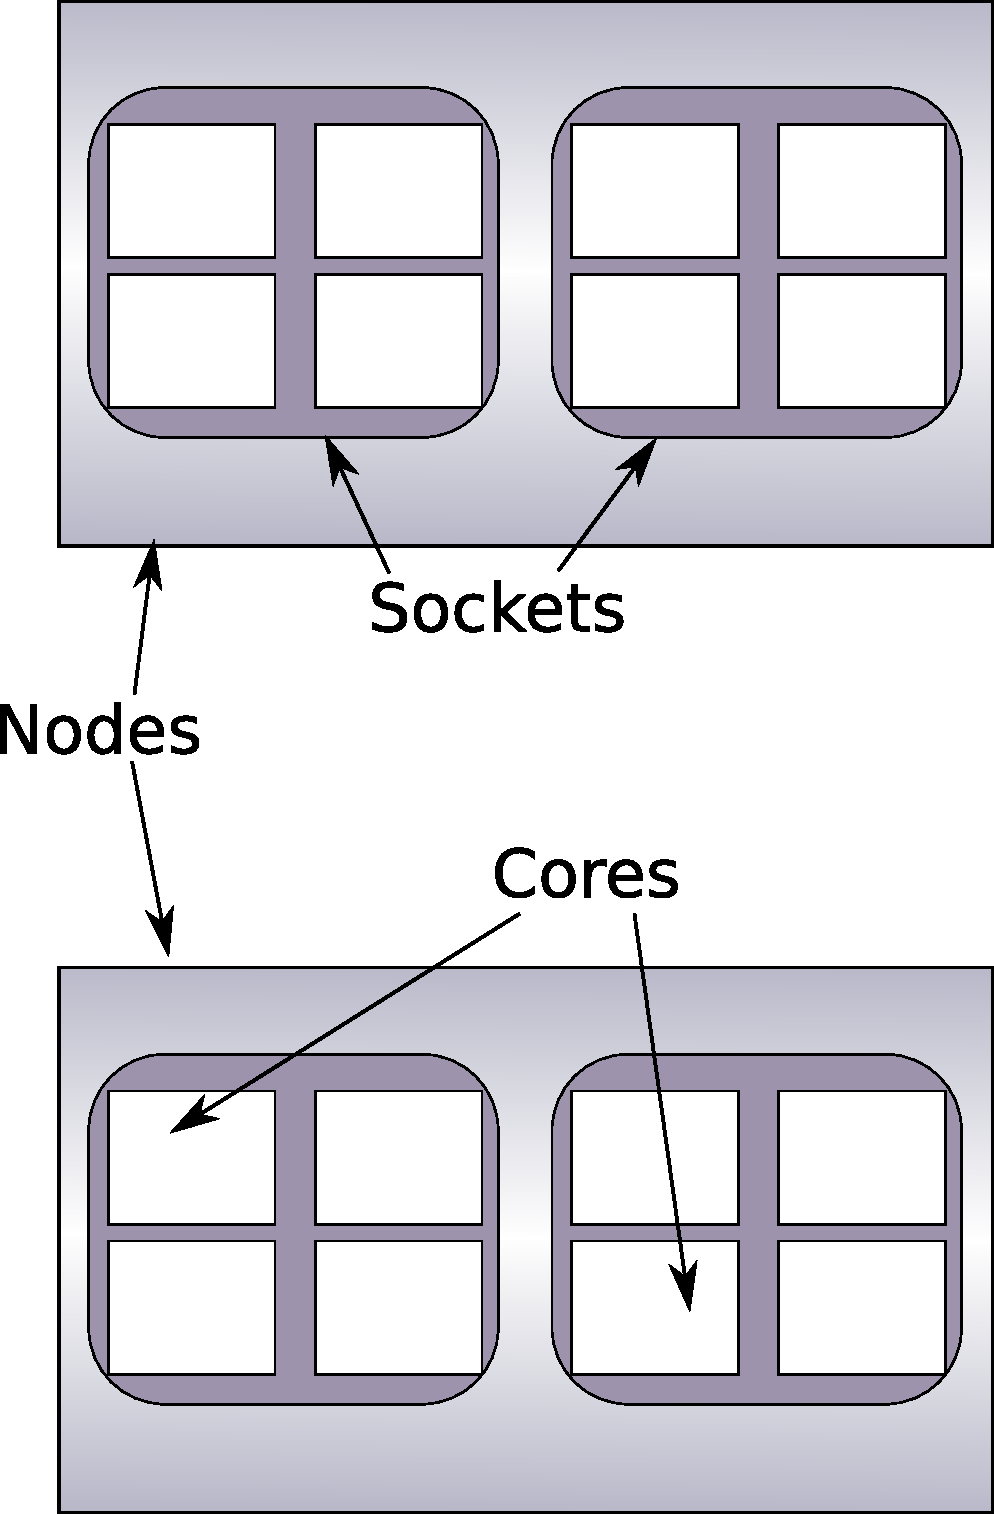
\includegraphics[height = 0.5\textheight]{cluster_hierarchy.pdf}
\caption{Schematic of a sample cluster architecture. This sample cluster consists of two nodes
(represented by the outermost rectangles), each of which has two sockets (rounded rectangles) with four
cores (small, white rectangles) per socket for a total of eight cores per node.}
\end{figure}

The different characteristics of inter- vs intra-node communication necessitates the use of different
techniques in parallelising code. \ambit\ employs two software libraries to achieve this: \textit{OpenMP} 
for distributing the workload among cores within a node and \textit{MPI} for distributing the workload
between nodes. These two methods of parallelism can be used in isolation or combined for a hybrid
approach. 

\section{MPI}
\label{sec:MPI}

MPI\footnote{\textit{Message Passing Interface} - technically a specification and standard rather than a
specific library. Implementations include OpenMPI, MPICH, and Intel MPI} provides a platform-independent
interface for communication between computing resources and allows for parallelism at either the core or
node level. Invoking a program with MPI spawns a number of independent \textit{processes} (the term which
we will use to refer to MPI parallelism throughout the rest of this section) which do not share resources
and cannot communicate outside of MPI directives, even if they reside on the same node. Each MPI process
runs its own copy of the \ambit\ code and requires its own set of variables, so there is some duplication
of resources (most importantly the CI matrix) between processes. Consequently, running multiple MPI
processes per node comes with some memory overhead, which limits the number of processes and parallel
speedup which is possible with a pure MPI approach.

To enable MPI support, \ambit\ must first be compiled with the \texttt{-D\_AMBIT\_USE\_MPI} compiler flag
(currently enabled by default on the Katana, Raijin and Peregrine clusters). Next, the MPI sections of
\ambit\ are only activated when the code is run with the either of the equivalent commands 
\texttt{mpirun} or \texttt{mpiexec}:

\begin{verbatim}
mpirun [-np <N>] <ambit>
\end{verbatim}

where \texttt{<ambit>} is the command and arguments you would usually use to run \ambit. Note that
\texttt{mpirun} will not always be available by default on clusters which employ a \textit{module-based}
system to manage software; it may be necessary to load the appropriate MPI module (e.g. OpenMPI) before
running \ambit\ in MPI-mode.

The \texttt{-np} option is optional (as indicated by the square brackets) and indicates the number of MPI
processes to spawn. If it is left out then MPI will make as many processes as there are available cores
across all nodes (i.e. a job with 2 nodes and 4 cores per node will spawn 8 MPI processes unless
otherwise specified with the \texttt{-np} option).

If your cluster/job scheduler allows you to request a specific number of nodes and cores per node
than the above command is all that is necessary to run \ambit\ with MPI. However, if the job scheduler
only allows requests for cores (NCI's \textit{Raijin} cluster schedules jobs this way) then it is still
possible to limit the number of MPI processes per node via command-line arguments to mpirun. The
\texttt{--map-by <resource>} option specifies how to distribute the generated MPI processes among
available computational resources.

The \texttt{--map-by} option requires at least the type of resource to ``map'' the processes to
(essentially, the level of granularity of control we want over how MPI distributes processes), which can
be node, socket or core\footnote{There are plenty of other options as well, which are beyond the
scope of this guide. Consult the man page if you're interested.}. If this option is used then the
\texttt{-np} option \textit{must} also be specified. Additionally, \texttt{--map-by} accepts
additional arguments specifying the number of processes to allocate, \texttt{ppr}, to each resource 
according to the pattern:

\begin{verbatim}
mpirun -np <N> --map-by ppr:<procs_per_resource>:<resource> <ambit>
\end{verbatim}

As a concrete example, suppose we want to spawn 4 processes per node on our model cluster shown in 
figure \ref{fig:cluster_hierarchy}. In this case, the command:

\begin{verbatim}
mpirun -np 8 --map-by ppr:4:node <ambit>
\end{verbatim}

This is a very coarse-grained level of control though, as MPI is free to spawn processes \emph{anywhere} 
on the node. This can be useful if the cluster is busy, as it allows \ambit\ to ``share'' the nodes with
other running jobs by placing the processes wherever is available. However, if the processes are spawned
across multiple sockets on the nodes, as shown in figure \ref{fig:MPI_map-by_node}, then this may degrade
performance, as it is considerably faster to pass messages
between cores on the same socket than it is to communicate across sockets.

\begin{figure}
\label{fig:MPI_map-by_node}
\centering
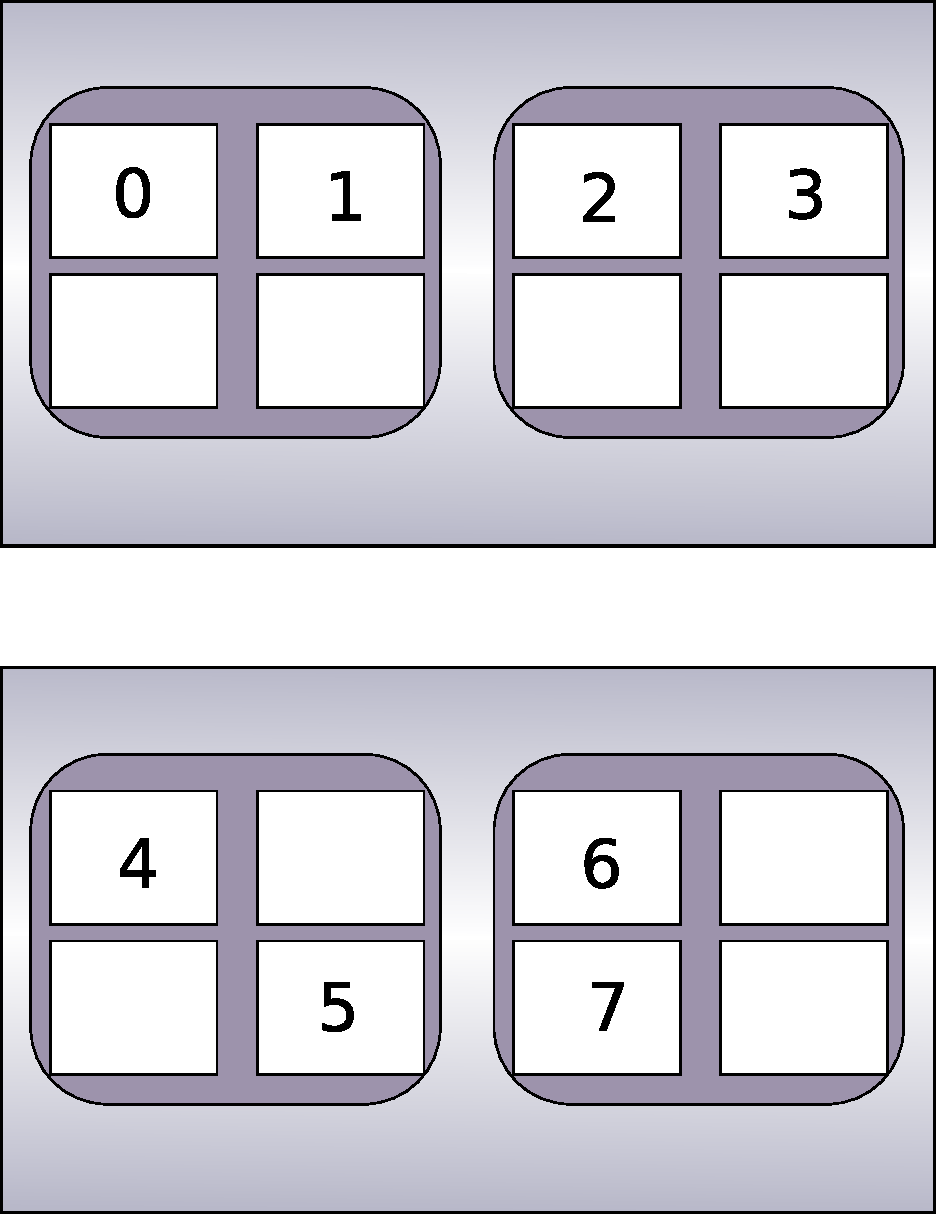
\includegraphics[height = 0.5\textheight]{MPI_map-by-node.pdf}
\caption{One possible distribution of MPI processes when using \texttt{--map-by ppr:4:node}. The
processes are distributed across sockets on the nodes, which may degrade performance due to the
difference in communication speed within sockets vs across sockets.}
\end{figure}

To overcome this issue, we can instead instruct MPI to map processes at the socket level by using:

\begin{verbatim}
mpirun -np 8 --map-by ppr:4:socket <ambit>
\end{verbatim}

This will still spawn 4 processes per node, but now the processes on a node will all be located on the
same socket, decreasing communication latency (provided only 4
cores per node have been requested). One possible distribution of processes for this mapping is shown in 
figure \ref{fig:MPI_map-by_socket}.

\begin{figure}
\label{fig:MPI_map-by_socket}
\centering
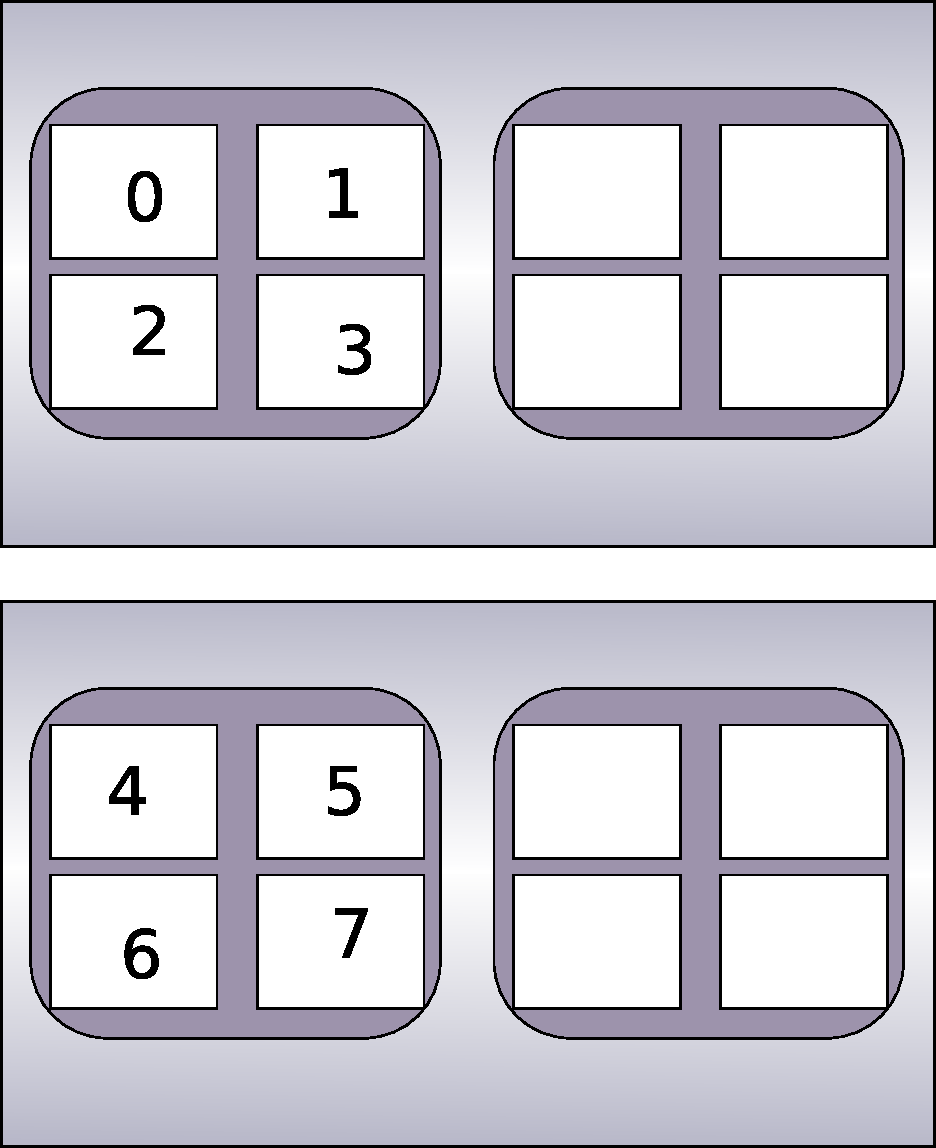
\includegraphics[height = 0.5\textheight]{MPI_map-by_socket.pdf}
\caption{One possible distribution of MPI processes when using \texttt{--map-by ppr:4:socket}. All
processes on a node are bound to the same socket, which can reduce communication latency and increase
performance.}
\end{figure}

Finally, it is also possible to map MPI processes by core, which will map the processes to whichever
cores are available without regard for node or socket. This is the default behaviour for most
current implementations of MPI\footnote{Binding/mapping processes by core is the default behaviour for
OpenMPI versions 1.7.x and above.} and is functionally identical to running \texttt{mpirun} without any
options.

\section{OpenMP}
\label{sec:OpenMP}
As previously mentioned, all cores within a node have access to a shared memory pool, so it is not
necessary to employ explicit message passing to distribute the workload. Consequently, we employ
\textit{shared-memory parallelism} via the \textit{OpenMP} library when running \ambit\ in parallel
\emph{within} a node. OpenMP employs the \textit{fork-join} model of parallelism. The code runs as a 
single \textit{thread} until it encounters a section (such as a subroutine or loop) which the programmer 
has declared should be run in parallel, at which point the program spawns multiple threads
which draw from a common pool of memory\footnote{At least, all OpenMP threads created by the same MPI 
process share memory. As we'll see, a hybrid MPI+OpenMP program can result in multiple ``groups'' of 
OpenMP threads executing on a single node, which share memory within groups spawned by the same process, 
but not between different groups} and distribute the work in the parallel section between them. 

In addition to OpenMP, \ambit\ can optionally make use of Intel's \textit{Math Kernel Library} 
(\textit{MKL}) to automatically parallelise certain linear algebra operations\footnote{Only operations 
with relatively moderate overhead are parallelised via MKL; the huge eigenvalue problems required by the
CI algorithm employ a different, more specialised algorithm instead.}. MKL's internal subroutines also
employ shared-memory parallelism, so all of the same performance concerns which apply to OpenMP also
apply to MKL.

By default, OpenMP attempts to guess how many threads to spawn upon entering a parallel region based on
the processor architecture the program is running on. This can give poor performance when running hybrid
MPI+OpenMP code, however, so it is usually best to manually specify the number of OpenMP/MKL threads to
use. This is achieved through setting the environment (e.g. bash) variables \texttt{OMP\_NUM\_THREADS} 
and \texttt{MKL\_NUM\_THREADS} by including the following lines in the job-script used to run \ambit:

\begin{verbatim}
export OMP_NUM_THREADS=<num_OpenMP_threads>
export MKL_NUM_THREADS=<num_MKL_threads>
\end{verbatim}

Note that if \texttt{MKL\_NUM\_THREADS} is not defined then MKL will use the same number of threads as 
OpenMP; this is a sensible default, so it is usually sufficient to only specify 
\texttt{OMP\_NUM\_THREADS}. 

To enable OpenMP support, \ambit\ must first be compiled with the \texttt{-D\_AMBIT\_USE\_OPENMP} compiler
flags and \texttt{OMP\_NUM\_THREADS} must be defined \emph{before} running \ambit. Additionally, MKL's
internal parallelism can be enabled by first compiling and linking \ambit\ against MKL libraries%
\footnote{The details of this are beyond the scope of this guide. Consult your cluster's documentation or
IT people for more details.} and passing the \texttt{-D\_EIGEN\_USE\_MKL\_ALL} flag during compilation.
Once \ambit\ has been compiled with the correct options and at least \texttt{OMP\_NUM\_THREADS} has been
defined, \ambit\ will use OpenMP parallelism without requiring any additional command line options (i.e.
simply run \ambit\ as you would normally).

OpenMP is very forgiving when it comes to performance issues and we have tried to ensure that \ambit
\textit{scales} well as more cores/threads are added. Performance will be drastically reduced if you
request more threads than there are available cores, but provided this condition is not met it is
generally safe to request as many OpenMP threads as there are available cores.

Additionally, a specific thread mapping (i.e. how to distribute threads across cores)
\texttt{KMP\_AFFINITY} is used to request a specific thread mapping, or
\textit{affinity}, which dictates where to place threads on the node and can have the values 
\texttt{compact}, \textit{scatter} or \textit{none}. \textit{Compact} mapping ensures consecutive 
threads are placed ``close'' together on the node (i.e. OpenMP will try to place threads on the same 
socket), as shown in figure \ref{fig:omp_compact}. 
\textit{scatter} indicates threads should be evenly distributed between sockets on a node, as shown in
figure \ref{fig:omp_scatter}.
Lastly, a value of \textit{none} indicates that the OpenMP runtime should automatically decide where to 
place threads.

Not requesting any affinity \emph{may} allow threads to migrate between cores as \ambit\ 
is running, which may degrade performance. Compact and scatter ensure threads stay bound to a specific
core for the lifetime of the calculation and only differ when running with fewer 
threads than there are available cores on a node. Even then these two affinities only differ 
substantially in memory access latency\footnote{Specifically, all cores on a
socket share a single memory bus, so highly memory intensive calculations may saturate the bus if all
threads are bound to a single socket. Conversely, it is expensive to communicate across sockets, so
computation intensive jobs may \emph{benefit} from all having threads bound to a single socket. The only
way to determine which affinity will give optimal performance for a specific job is to try both and 
compare}. Consequently, it is usually good practice to explicitly request a thread affinity of either 
compact or scatter, the choice of which only matters when running \ambit\ with fewer than the available
number of cores on a node. This is achieved by adding the following line to the job script used to run
\ambit:

\begin{verbatim}
export KMP_AFFINITY=<affinity>
\end{verbatim}

\begin{figure}
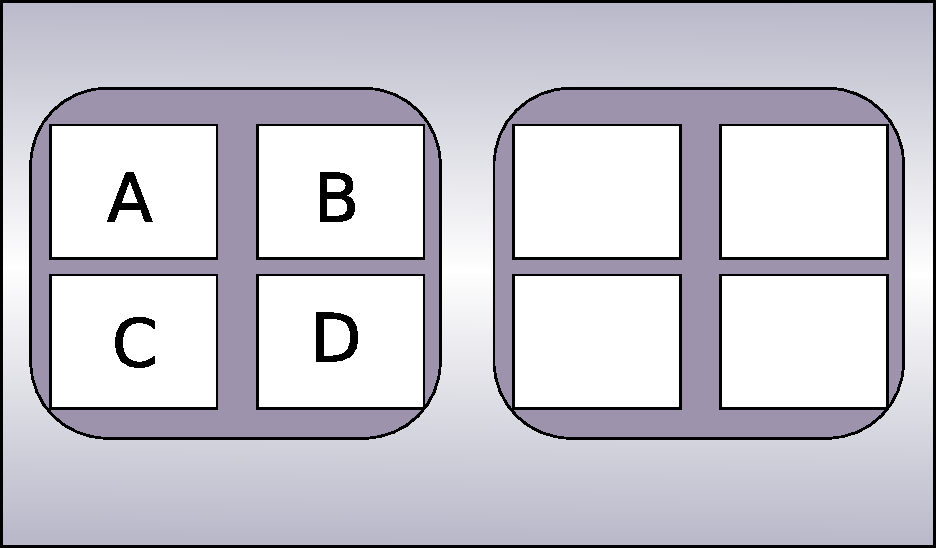
\includegraphics[width=0.5\textwidth]{omp_compact.pdf}
\caption{Schematic representation of OpenMP compact thread mapping with four threads (labelled A-D) on
a single node of the model cluster shown in figure \ref{fig:cluster_hierarchy}.}
\label{fig:omp_compact}
\end{figure}

\begin{figure}
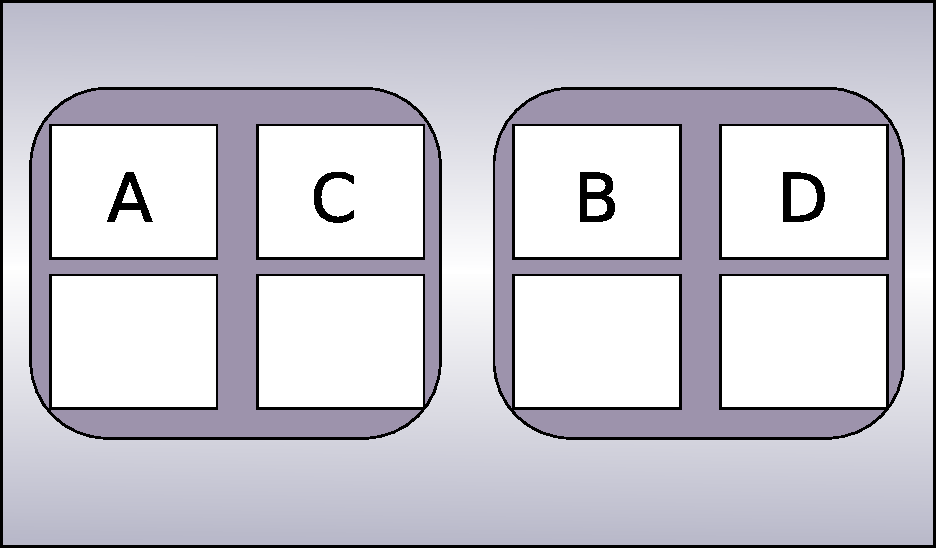
\includegraphics[width=0.5\textwidth]{omp_scatter.pdf}
\caption{Schematic representation of OpenMP scatter thread mapping with four threads (labelled A-D) on
a single node of the model cluster shown in figure \ref{fig:cluster_hierarchy}.}
\label{fig:omp_scatter}
\end{figure}

\begin{comment}
As a point of comparison, figure \ref{fig:OMPvsMPI} provides a comparison of the run times of \ambit\ (for
a mid-sized Sn$^{10+}$ calculation) using pure OpenMP as compared to pure MPI on UNSW's Katana cluster. 
In each case, the number of processes/threads starts at one and is increased to 16 across a single, 
16-core node on katana. Both cases  demonstrate clear parallel scaling (i.e. the run time steadily 
decreases as more resources are added), but the pure OpenMP approach completes in significantly less 
time than MPI - OpenMP running over 16 cores completes in $\sim 1/5$ of the time taken by the pure MPI 
approach.

\begin{figure}
\label{fig:OMPvsMPI}
\includegraphics{OMPvsMPI}
\end{figure}

This is a clear demonstration of the advantages of OpenMP over MPI when distributing workloads across a 
single node. 
\end{comment}
In summary, if your job fits on a single node (i.e. the CI matrix is not larger than the 
memory possessed by a single node) then it is almost always preferable to run \ambit\ with OpenMP rather 
than MPI.

\section{Hybrid OpenMP + MPI}
\label{sec:hybrid}

\ambit\ also supports a hybrid method of parallelism, exploiting the complementary performance aspects of
MPI and OpenMP to provide good scaling across multiple cluster nodes. We employ MPI to coordinate and
distribute work across nodes, while parallelism \emph{within} each node is handled by OpenMP. This allows
for jobs to be spread across multiple nodes (for example, if the CI matrix is too large to fit in the
memory of a single node), while maintaining as much of the speedup due to shared memory multithreading as
possible. 

Since it is fastest to use OpenMP within a node, it is generally ideal to run exactly one MPI process per
node and allow those process to spawn as many OpenMP threads as required\footnote{It may be desirable 
to run one MPI process per \emph{socket} for calculations where memory bandwidth is the bottleneck (as 
cores on a socket generally share a single memory bus) or when running on ccNUMA nodes (where latency in
accessing memory across sockets and cache-thrashing can cause significant slowdowns). In these cases,
always do a small test run with one MPI process per node and only test with one process per socket if
performance in the former case is unacceptably bad}. Both process and thread
creation are handled by the MPI library; exact details of which differ between implementations, which 
include \textit{OpenMPI}, \textit{MPICH} and \textit{Intel MPI}. This section will only focus on the
specifics of hybrid parallelism under OpenMPI, as it provides the most finely-grained control over how to
distribute MPI processes and OpenMP threads. While it is possible to use other MPI implementations with
\ambit\footnote{This requires recompiling \ambit\ and linking against the desired MPI library, which we
do not recommend for most users.}, there can be significant performance issues when using the Intel MPI
library, so we recommend you stick with OpenMPI unless there are significant reasons not to.

As described in section \ref{sec:OpenMP}, the \texttt{OMP\_NUM\_THREADS}
environment variable must be set before running \ambit. However, it is also necessary to be ``exported''
to all MPI processes by passing \texttt{-x OMP\_NUM\_THREADS} as an argument to \texttt{mpirun}. In 
addition to the \texttt{--map-by} command introduced in section
\ref{sec:MPI}, we must also specify the number of \textit{processing elements} (OpenMP threads) each MPI 
process should produce by extending \texttt{--map-by} with the \texttt{pe} option. The \texttt{mpirun}
command for hybrid mode has the following structure:

\begin{verbatim}
export OMP_NUM_THREADS=<num_threads>
...
mpirun -np <num_nodes> --map-by ppr:1:node:pe=<num_threads> \
-x OMP_NUM_THREADS <ambit>
\end{verbatim}

As previously stated, the number of threads must be specified twice in this command: once to tell 
OpenMPI how many threads to expect and then again to tell OpenMP how many threads to actually spawn. This
is inconvenient, but unfortunately there is currently no reliable way to have either OpenMP or OpenMPI 
handle this automatically.

As a more concrete example, 
consider the model cluster introduced in figure \ref{fig:cluster_hierarchy}. The command to run \ambit\ 
with one MPI process per node and 8 OpenMP threads per process is:

\begin{verbatim}
export OMP_NUM_THREADS=8
...
mpirun -np 2 --map-by ppr:1:node:pe=8 -x OMP_NUM_THREADS <ambit>
\end{verbatim}

This will result in a process and thread distribution similar to figure \ref{fig:hybrid_per_node}.

\begin{figure}
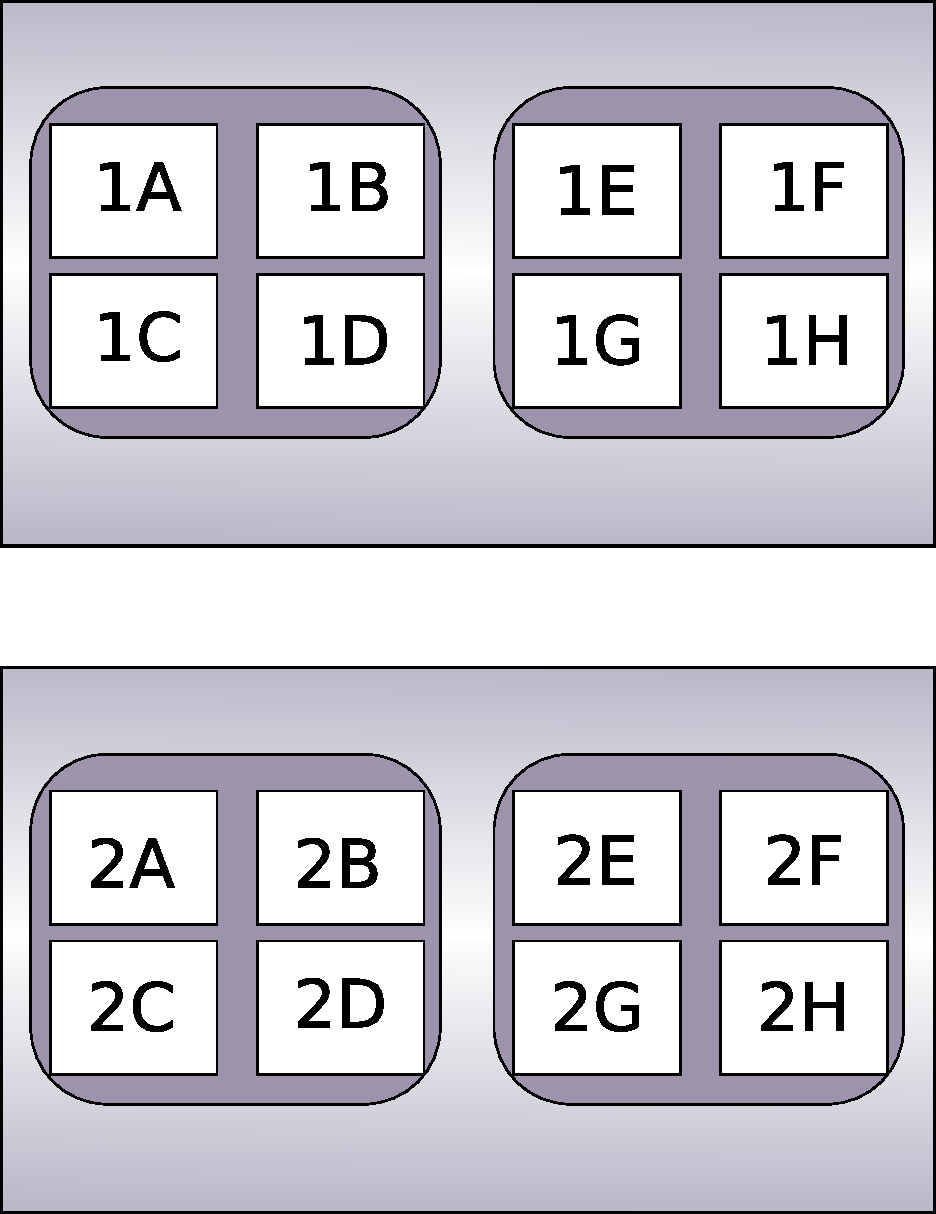
\includegraphics[height=0.5\textheight]{hybrid_map_by_node.pdf}
\caption{One possible distribution of MPI processes and OpenMP threads running with 1 process per node.
MPI processes are represented by numbers while OpenMP threads are represented by capital letters 
(e.g. 2C refers to the third thread spawned by process 2)}
\label{fig:hybrid_per_node}
\end{figure}

%%%%%%%%%%%%%%%%%%%%%%%%%% Mapping MPI processes by node %%%%%%%%%%%%%%%%%%%%%%%%%%%%%%%
\begin{comment}
Alternatively, the command to run with one process per \textit{socket} is:

\begin{verbatim}
export OMP_NUM_THREADS=4
...
mpirun -np 4 --map-by ppr:1:socket:pe=4 -x OMP_NUM_THREADS <ambit>
\end{verbatim}

and would result in a mapping similar to figure \ref{fig:hybrid_per_socket}. 

\begin{figure}
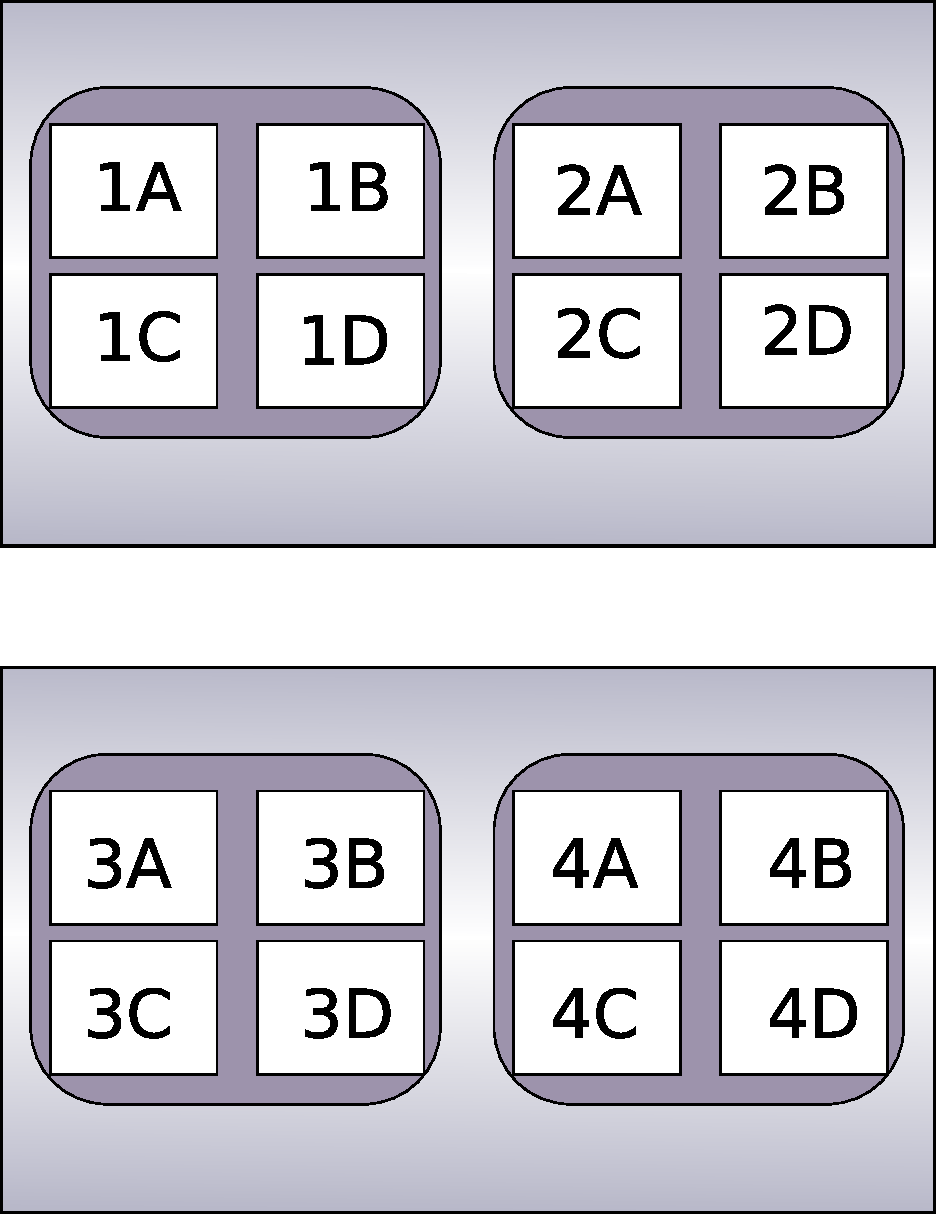
\includegraphics[height=0.5\textheight]{hybrid_map_by_socket.pdf}
\caption{One possible distribution of MPI processes and OpenMP threads running with 1 process per 
socket. MPI processes are represented by numbers while OpenMP threads are represented by capital letters 
(e.g. 2C refers to the third thread spawned by process 2)}
\label{fig:hybrid_per_socket}
\end{figure}

Additionally, we can directly inspect the mapping of processes and threads at run-time via options to
both OpenMPI and OpenMP. First, the \texttt{--report-bindings} option to \texttt{mpirun} will print the
``location'' of each MPI process spawned by the calculation to \texttt{stderr}. Similarly, code compiled
with the Intel OpenMP library (currently the case on \textit{Katana} and \textit{Raijin}) can be
instructed to print the mapping of OpenMP threads, also to \texttt{stderr}, by setting the environment
variable \texttt{KMP\_AFFINITY}. In addition to the affinity/mapping options specified in section
\ref{sec:OpenMP}, \texttt{KMP\_AFFINITY} can also take the \texttt{verbose} parameter, which will print
the thread affinity to \texttt{stderr}. Consequently, we can use the output redirection capabilities of
bash (i.e. the > symbol) to collect both of these mappings into a single file, with a job script of the
form:
\end{comment}
%%%%%%%%%%%%%%%%%%%%%%%%%%%%%%%%%%%%%%%%%%%%%%%%%%%%%%%%%%%%%%%%%%%%%%%%%%%%%%%%%%%%%%

The above commands can be extended to as many nodes as required by only changing the number of
requested MPI processes (via the \texttt{-np} option to \texttt{mpirun}); the OpenMP specific options
(\texttt{OMP\_NUM\_THREADS} and the \texttt{pe} option to \texttt{mpirun}) do not need to be changed
unless \ambit\ will be run on multiple, heterogeneous nodes with different numbers of available cores.
This usage case is beyond the scope of this guide, so ask the IT support for your cluster if you need to 
run \ambit\ in this configuration.

\section{Cluster specific information}
\label{sec:cluster_specific}
\subsection{Raijin}
All modes of \ambit\ parallelism currently work on Rajiin with no requirements or special commands above 
and beyond what has been mentioned so far in this guide. In terms of hardware, all currently available 
nodes in the \textit{normal} and \textit{express} queues in have two sockets with 8 cores per socket, 
for a total of 16 cores per node. Each node has a total of 128GB of memory shared between sockets,
however the job scheduler prioritises jobs which require a low memory amount of memory per node so it is 
advisable not to request more memory than is strictly required. It is also important to note that the
total requested amount of memory for a job is spread equally between all nodes, so requesting
\texttt{\#PBS -l mem=60GB} on a 3-node job will result in 20GB of available memory per node, \emph{not}
60GB per node.

In addition, the job scheduling system has slightly different methods of requesting jobs on one node 
compared to jobs requiring multiple nodes. For one node, it is possible to specify an arbitrary number of
cores (e.g. \texttt{\#PBS -l cores=[1-16]}) and the job scheduler will attempt to allocate all cores on 
the same node. For greater than one node (i.e. \texttt{\#PBS -l cores=[>16]}, it is only possible to 
request cores in multiples of 16 (so requesting two nodes requires \texttt{\#PBS -l cores=32}). It is 
not possible to request multiple nodes in any other manner.

\subsection{Katana}

Currently, it is not possible to run hybrid OpenMP+MPI jobs on Katana: attempting to use more than one
MPI process with OpenMP causes \ambit\ to hang when diagonalising the Hamiltonian Matrix\footnote{This is
achieved via the Davidson algorithm, which we have explicitly parallelised via MPI and rely on the
automatic shared memory parallelism in the \textit{Eigen} linear algebra library.}. The source of this
bug is still currently unknown, so for now it is necessary to run \ambit\ in either pure OpenMP mode if
the job will fit on one node or pure MPI if more than one node is required.

The Katana nodes available to the Atomic Physics group fall into two groups:

\begin{itemize}
\item 2 sockets per node, 8 cores per socket for 16 cores per node; 128GB memory ($\times 4$)
\item 2 sockets per node, 6 cores per socket for 12 cores per node; 96GB memory ($\times 2$)
\end{itemize}

The above nodes are exclusively owned by the Berengut research group, so there is less penalty for
overestimating job resource usage than on Raijin.

\section{Further reading}

The following resources may be useful when troubleshooting hybrid parallelism in \ambit:
\begin{itemize}
\item \href{https://opus.nci.org.au/display/Help/Hybrid+MPI+OpenMP}{Raijin User Guide: Hybrid MPI+OpenMP
(NCI)} - Contains general advice on running programs using pure MPI and hybrid OpenMP+MPI parallelism, 
as well as example PBS batch scripts. Batch scripts are specific to Raijin, but most advice is generally
applicable across clusters.

\item \href{https://opus.nci.org.au/display/Help/How+to+Debug+Parallel+Programs}{Raijin User Guide: How
to Debug Parallel Programs} - Provides advice and working examples for debugging MPI parallel jobs on
Raijin. Can be useful for locating performance bottlenecks as well as bugs.

\item \href{https://software.intel.com/en-us/articles/intel-mkl-link-line-advisor/}{Intel MKL Link Line
Advisor} - Online tool to determine which compiler flags to use with \ambit\ to enable MKL functionality.

\item \href{https://www.open-mpi.org/faq/}{OpenMPI FAQ} - Provides general advice for compiling and
running MPI programs on a variety of cluster and software environments.
\end{itemize}

\chapter{User input options}
\label{chap:input}

\section{Introduction}

This chapter lists and outlines the syntax of input options accepted by \ambit. The input options are
grouped by their ``prefix'', loosely corresponding to different components of the calculation
(Hartree-Fock, CI, etc), with the exception of a few general-purpose ``ungrouped'' options which have no
prefix. Options can be specified in two ways:
\begin{itemize}
\item Directly, via the command-line. When invoking the \texttt{ambit} executable, command-line options 
may be passed as \texttt{Prefix/Option}.
\item Through an input file. Input files are plain text files containing one or more options to be
passed to \ambit. Options in the input file are grouped into sections according to a prefix with the
syntax:

\texttt{Option1}\\
\texttt{[Prefix1]}\\
\texttt{Option2}\\
\texttt{[Prefix2]}\\
\texttt{Option3}

All options appearing before the first prefix are treated as ``ungrouped'', while all options between
two prefixes are treated as belonging to the first option. Consequently, \texttt{Option1} in the above
snippet will have no prefix, while \texttt{Option2} and \texttt{Option3} are equivalent to
\texttt{Prefix1/Option2} and \texttt{Prefix2/Option3}, respectively.

Input files are specified on the command line with the \texttt{-f} option; if this is not present,
\ambit\ will search the command line arguments for a filename with the \texttt{.input} extension and
automatically read input options from that file. Consequently, the following two invocations are
equivalent:

\texttt{ambit -f file.input}\\
\texttt{ambit file.input}
\end{itemize}

Currently, misspelled or erroneous arguments are not automatically handled by \ambit\ 
and will be either be ignored (for typos) or cause the corresponding part of the calculation to fail 
(for errors or incorrect arguments).

\subsection{Conventions used throughout this chapter}

Each section of this document corresponds to a prefix (except for section \ref{sec:ungrouped}, which
contains ungrouped options), with the options belonging to that prefix outlined at the beginning of the
section. 

Additionally, the input options may either take an argument (specified after an ``=''), or are binary
``flags'' which do not take arguments and control \ambit\ by whether or not they are specified. This
distinction is reflected in the syntax and naming conventions of arguments. Options requiring an
argument are written in CamelCase and have the form \texttt{InputOption=Argument}, where the argument
can be either a numeric value (an integer or a real number) or a text string encased in single- or
double-quotes. Quotes may be omitted only in the special case of a string-type argument which is a
single word, in which case \ambit\ will automatically treat the argument as a string (multi-word
arguments are never automatically converted). Input flags, on the other hand, are written in lower case 
and have the form \texttt{{-}{-}flag-option} (note the two leading-dashes). 

Definitions have the following form:

\texttt{OptionName, Synonym} \uline{Type of arguments}[Default value]
\begin{adjustwidth}{1cm}{}
Short description of what the option does.
\end{adjustwidth}

Finally, the value of all numerical parameters must be given in atomic units unless otherwise specified.

\section{Multirun Options}

\label{sec:multirun}

It is sometimes necessary to run multiple almost identical CI+MBPT calculations which differ only in
some varying parameter, such as the nuclear mass or radius in field-shift calculations. To facilitate
this use-case, \ambit\ supports multiple runs via the \texttt{Multirun} ungrouped input option, which
accepts a string containing the parameter to vary. The varying parameters values are then provided via 
the usual input options, except they must be given as a list of values the parameter may take. For 
example:

\texttt{Multirun = 'AlphaSquaredVariation'}
\texttt{AlphaSquaredVariation = '-0.1, 0.0, 0.1'}

will perform three runs with $\alpha^2 \to (1 + \Delta)\alpha^2$ for $\Delta = -0.1, 0.0, 0.1$.

The resulting energy levels and transition matrix elements are for each run are all grouped according to
$J^{\pi}$ symmetry and printed to standard output. And example output file might look like:

\begin{verbatim}

AlphaSquaredVariation = -0.1
 Number of CSFs = 332 x 15; Finding solutions using Davidson...
    nloops=12
Solutions for J = 1, P = even (N = 332):
0: -0.63475278    -139312.133015 /cm
             3s1 4s1  82.9916%
             3s1 5s1  14.3713%
             3p1 4p1  1.9466%
    g-factor = 2

1: -0.60239174    -132209.70548 /cm
             3s1 3d1  57.1468%
             3s1 4d1  41.1429%
    g-factor = 0.50001

AlphaSquaredVariation = 0
 Number of CSFs = 332 x 15; Finding solutions using Davidson...
    nloops=12
Solutions for J = 1, P = even (N = 332):
0: -0.63484229    -139331.777879 /cm
             3s1 4s1  82.9909%
             3s1 5s1  14.3737%
             3p1 4p1  1.9449%
    g-factor = 2

1: -0.60247228    -132227.38166 /cm
             3s1 3d1  57.1408%
             3s1 4d1  41.1492%
    g-factor = 0.50001

AlphaSquaredVariation = 0.1
 Number of CSFs = 332 x 15; Finding solutions using Davidson...
    nloops=12
Solutions for J = 1, P = even (N = 332):
0: -0.63493188    -139351.440654 /cm
             3s1 4s1  82.9902%
             3s1 5s1  14.3760%
             3p1 4p1  1.9432%
    g-factor = 2

1: -0.60255289    -132245.074402 /cm
             3s1 3d1  57.1348%
             3s1 4d1  41.1555%
    g-factor = 0.50001

\end{verbatim}

Each run has its own separate basis, integral and levels files, which are distinguished by a suffix
indicating the run number, such as \texttt{<ID>\_0.basis}, \texttt{<ID>\_1.basis}, 
\texttt{<ID>\_2.basis} for the above calculation. The run number is always 0 if no multirun options are
used.

\section{Ungrouped options}
\label{sec:ungrouped}

\texttt{ID} \uline{String}
\begin{adjustwidth}{1cm}{}
(Mandatory) String identifying the calculation. This string will be used to generate the names of 
temporary files, as well as stored basis functions, MBPT integrals and energy levels 
(allowing calculations to be reused or interrupted and resumed).
\end{adjustwidth}

\texttt{Z} \uline{Integer}
\begin{adjustwidth}{1cm}{}
(Mandatory) Atomic number of the target system. 
\end{adjustwidth}

\texttt{-f} \uline{filename}
\begin{adjustwidth}{1cm}{}
Filename (and path) of input file containing options to be passed to \ambit. 
\end{adjustwidth}

\texttt{NuclearInverseMass} \uline{Real}
\begin{adjustwidth}{1cm}{}
Inverse mass of the nucleus in atomic units. Used when calculating mass shift.
\end{adjustwidth}

\texttt{NuclearRadius} \uline{Real}
\begin{adjustwidth}{1cm}{}
Radius parameter of a Fermi distribution for nuclear charge. This value is 
used to compute the nuclear RMS radius, which is not specified directly. If neither 
\texttt{NuclearRadius} or \texttt{NuclearThickness} are set then the nucleus is treated as a point 
charge.
\end{adjustwidth}

\texttt{NuclearThickness} \uline{Real}
\begin{adjustwidth}{1cm}{}
Specifies the density parameter of a Fermi distribution for nuclear charge. 
If neither \texttt{NuclearRadius} or \texttt{NuclearThickness} are set then the nucleus is treated as a 
point charge.
\end{adjustwidth}

\texttt{AlphaSquaredVariation} \uline{Real}
\begin{adjustwidth}{1cm}{}
Vary the value of the fine-structure constant by some factor $\Delta$ such that 
$\alpha^2 \to (1 + \Delta)\alpha^2$. 
\end{adjustwidth}

\texttt{AngularDataDirectory} \uline{String}
\begin{adjustwidth}{1cm}{}
Alternative directory used to store and read angular data files. This option overrides the angular data
directory set by the \texttt{-DANGULAR\_DATA\_DIRECTORY} compile-time option.
\end{adjustwidth}

\texttt{LevelDirectory} \uline{String}
\begin{adjustwidth}{1cm}{}
Directory to store energy levels when using \texttt{CI/{-}{-}memory-saver}.
\end{adjustwidth}

\texttt{-s[123]} 
\begin{adjustwidth}{1cm}{} 
Specifies the number of particles to include in MBPT diagrams. Any combination of 1, 2 or 3 may follow 
\texttt{s}, so e.g. \texttt{-s1} will generate one-body diagrams, while \texttt{-s123} will generate all 
one-, two- and three-body diagrams. No MBPT corrections will be calculated if this flag is not present.
\end{adjustwidth}

\texttt{--no-new-mbpt}
\begin{adjustwidth}{1cm}{} 
Do not calculate any new MBPT integrals. Any integrals saved in \texttt{.int} files will still be read, 
but integrals which have been requested, but not present in the \texttt{.int} files will not be
calculated.
\end{adjustwidth}

\texttt{--check-sizes}
\begin{adjustwidth}{1cm}{}
Calculate and print the number of Coulomb and MBPT integrals, as well as the size of the CI matrix for
each symmetry $J^{\pi}$. Calculations with this option will also generate the angular data (if needed),
which can be computationally expensive and often requires the calculation to be run with OpenMP
parallelism. Used to determine the size of a calculation before running it in full.
\end{adjustwidth}

\texttt{-c, --clean}
\begin{adjustwidth}{1cm}{}
Run the calculation without reading pre-calculated basis functions, MBPT integrals or energy levels (a
``clean run'').
\end{adjustwidth}

\texttt{-p, --print-basis}
\begin{adjustwidth}{1cm}{}
Print basis orbitals in plain (ASCII) text. Orbitals are currently always written to
\texttt{Orbitals.txt}, which is overwritten if it already exists.
\end{adjustwidth}

\texttt{--ci-complete, --CI-complete}
\begin{adjustwidth}{1cm}{}
Do not calculate extra energy levels if more levels are requested via \texttt{CI/NumSolutions} than
exist in the precalculated levels file.
\end{adjustwidth}

\texttt{--no-ci, --no-CI}
\begin{adjustwidth}{1cm}{}
Do not do any CI calculations, such as when doing one-electron calculations.
\end{adjustwidth}

\texttt{{-}{-}configuration-average}
\begin{adjustwidth}{1cm}{}
Use configuration average energy when generating the CI matrix.
\end{adjustwidth}

\texttt{-h}
\begin{adjustwidth}{1cm}{}
Print a help message.
\end{adjustwidth}

\texttt{--version}
\begin{adjustwidth}{1cm}{}
Print \ambit\ version information. Output includes a version number, git branch, and date and time of 
compilation. This information is also printed in the output of all calculations.
\end{adjustwidth}

\texttt{-r} \uline{List of values}
\begin{adjustwidth}{1cm}{}
Select a subset of specified runs for this calculation. Only used when there are multiple runs specified
(see section \ref{sec:multirun}); the calculation will be repeated for each value specified in this
argument.
\end{adjustwidth}

\texttt{Multirun} \uline{String}
\begin{adjustwidth}{1cm}{}
Parameter to be varied when performing multiple runs. This is described in detail in section
\ref{sec:multirun}.
\end{adjustwidth}

\section{Lattice}

\texttt{NumPoints} \uline{Integer}[1000]
\begin{adjustwidth}{1cm}{}
Maximum number of points to include in the radial wavefunction lattice.
\end{adjustwidth}

\texttt{StartPoint} \uline{Real}[1.0e-6]
\begin{adjustwidth}{1cm}{}
Starting point of the lattice (in atomic units).
\end{adjustwidth}

\texttt{EndPoint} \uline{Real}[50.0]
\begin{adjustwidth}{1cm}{}
End point of the lattice (in atomic units).
\end{adjustwidth}

\texttt{--exp-lattice}
\begin{adjustwidth}{1cm}{}
Use a lattice with strictly exponential spacing, rather than the default hybrid linear-exponential
scheme. This changes the default value of \texttt{Lattice/NumPoints} to 300 and
\texttt{Lattice/StartPoint} to 1.0e-5.
\end{adjustwidth}

\texttt{H} \uline{Real}[0.05]
\begin{adjustwidth}{1cm}{}
Parameter determining the spacing between points along the lattice. Only used in conjunction with
\texttt{--exp-lattice}.
\end{adjustwidth}

\section{HF}

\texttt{N} \uline{Integer}
\begin{adjustwidth}{1cm}{}
(Mandatory) Number of electrons to include in the Hartree-Fock procedure.
\end{adjustwidth}
\texttt{Configuration} \uline{String} 
\begin{adjustwidth}{1cm}{}
(Mandatory) Nonrelativistic configuration to be used for the
Dirac-Fock calculations (can include valence as well as core electrons). The Fermi level can be specified
with a colon (`:'), orbitals above which will be included in the CI and MBPT valence space $P$. If no
Fermi level is specified it will default to immediately above the highest supplied orbital in this
argument. Additionally, Valence holes can only appear in shells with energy below the Fermi level.
                                                                               
As an example, the string \texttt{HF/Configuration = '1s2 2s2 2p6~:~3s1'} will include the configuration
1s$^2$ 2s$^2$ 2p$^6$ 3s$^1$, with 1s, 2s and 2p shells below and 3s above the Fermi level.
Configuration must have \texttt{HF/N} total electrons.
\end{adjustwidth}

\texttt{--breit} 
\begin{adjustwidth}{1cm}{}
Include effects of the Breit interaction.
\end{adjustwidth}
\texttt{--sms} 
\begin{adjustwidth}{1cm}{}
Include specific mass-shift operator (for use when calculating isotope shifts).
\end{adjustwidth}
\texttt{--nms} 
\begin{adjustwidth}{1cm}{}
Include normal mass-shift operator (for use when calculating isotope shifts).
\end{adjustwidth}
\texttt{--only-relativistic-nms} 
\begin{adjustwidth}{1cm}{}
Only include relativistic contribution to normal mass-shift operator.
\end{adjustwidth}
\texttt{--nonrelativistic-mass-shift}
\begin{adjustwidth}{1cm}{}
Only include non-relativistic contribution to a mass-shift operator.
\end{adjustwidth}

\texttt{--include-lower-sms}
\begin{adjustwidth}{1cm}{}
Include the lower-component of the wavefunction when using the non-relativistic specific mass-shift operator.
This can produce unphysical results, and is not recommended.
\end{adjustwidth}

Summary of mass shift options for relativistic and nonrelativistic operators:
\begin{adjustwidth}{1cm}{}
\begin{tabular}{|l|l|l|}
\cline{2-3}
\multicolumn{1}{c|}{} & Normal Mass Shift & Specific Mass Shift \\
\hline
Relativistic & \texttt{--nms} & \texttt{--sms} \\
\cline{2-2}
 & Only include relativistic contribution: & \\
 & \texttt{--nms} & \\
 & \texttt{--only-relativistic-nms} & \\
\hline
Nonrelativistic & \texttt{--nms} & \texttt{--sms} \\
 & \texttt{--nonrelativistic-mass-shift} & \texttt{--nonrelativistic-mass-shift} \\
\cline{3-3}
 & & Include lower part of Dirac spinors: \\
 & & \texttt{--sms} \\
 & & \texttt{--nonrelativistic-mass-shift} \\
 & & \texttt{--include-lower-sms} \\
\hline
\end{tabular}
\end{adjustwidth}

\texttt{--read-grasp0}
\begin{adjustwidth}{1cm}{}
(No longer used) Use lattice and basis orbitals from the output of a GRASP MCDF calculation.
\end{adjustwidth}

\texttt{--local-exchange}
\begin{adjustwidth}{1cm}{}
Use a local approximation to the HF exchange operator. This is faster than using nonlocal exchange, but
reduces accuracy. The type of local-approximation is specified by the value of \texttt{HF/Xalpha}, with
a default value of 1 (Dirac-Slater potential).
\end{adjustwidth}

\texttt{Xalpha} \uline{Real}[1.0]
\begin{adjustwidth}{1cm}{}
Specifies the type of local exchange potential. \texttt{Xalpha=1} corresponds to the Dirac-Slater
potential, \texttt{Xalpha=0.66} (2/3) corresponds to the Kohn-Sham potential and \texttt{Xalpha=0}
corresponds to the Core-Hartree potential.
\end{adjustwidth}

\subsection{HF/QED}
\texttt{--uehling}
\begin{adjustwidth}{1cm}{}
Include the Uehling (vacuum polarisation) QED correction.
\end{adjustwidth}

\texttt{--self-energy}
\begin{adjustwidth}{1cm}{}
Include the self-energy QED correction.
\end{adjustwidth}

\texttt{--use-nuclear-density}
\begin{adjustwidth}{1cm}{}
Use the nuclear density (rather than the default of nuclear radius) for nuclear contribution to Uehling 
corrections.
\end{adjustwidth}

\texttt{NuclearRMSRadius} \uline{Real}
\begin{adjustwidth}{1cm}{}
Nuclear RMS radius to use for nuclear contribution to Uehling corrections. Defaults to the value in 
\texttt{NuclearRadius} if unspecified.
\end{adjustwidth}

\texttt{--no-magnetic}
\begin{adjustwidth}{1cm}{}
Ignore the magnetic component of the self-energy correction, so only the electric (high- and
low-frequency) components are included. If no \texttt{QED/--no-electric} is also passed then the self-energy
correction will not be calculated.
\end{adjustwidth}

\texttt{--no-electric}
\begin{adjustwidth}{1cm}{}
Ignore the electric (high- and low-frequency) components of the self-energy correction, so only the
magnetic component is included. If no \texttt{QED/--no-magnetic} is also passed then the self-energy
correction will not be calculated.
\end{adjustwidth}

\texttt{--skip-offmass}
\begin{adjustwidth}{1cm}{}
Use an approximate method to calculate the radiative potential by taking the offmass term outside the self-energy integral.
Black magic, but it tends to work.
\end{adjustwidth}

\texttt{--use-electron-screening}
\begin{adjustwidth}{1cm}{}
Used to estimate the effect of electron screening of the nucleus (due to the charge density of the electrons)
on the radiative potential.
\end{adjustwidth}

\subsection{HF/Yukawa}
\texttt{Mass} \uline{Real}[1.0]
\begin{adjustwidth}{1cm}{}
Mass (in atomic units) of the particle coupled via the Yukawa interaction. Overrides any value set by
\texttt{Yukawa/MassEV} or \texttt{Yukawa/Rc}.
\end{adjustwidth}

\texttt{MassEV} \uline{Real}[1.0]
\begin{adjustwidth}{1cm}{}
Mass (in electron volts) of the particle coupled via the Yukawa potential. Not used if
\texttt{Yukawa/Mass} is specified.
\end{adjustwidth}

\texttt{Rc} \uline{Real}[1.0]
\begin{adjustwidth}{1cm}{}
Parameter determining the cutoff radius of the Yukawa interaction. Not used if \texttt{Yukawa/Mass}
or \texttt{Yukawa/MassEV} is specified.
\end{adjustwidth}

\texttt{Scale} \uline{Real}[1.0]
\begin{adjustwidth}{1cm}{}
Scale-factor for the Yukawa interaction.
\end{adjustwidth}

\subsection{HF/AddLocalPotential}

\texttt{Filename} \uline{String}
\begin{adjustwidth}{1cm}{}
Include a custom, local HF potential contained in \texttt{Filename}. Imported file must be plain-text
and contain a list of pairs of radial points $R$ and corresponding potentials $V(R)$, with exactly one
pair per line. All \texttt{HF/AddLocalPotential} options are skipped if no \texttt{Filename} is provided.
\end{adjustwidth}

\texttt{Scale} \uline{Integer}[1.0]
\begin{adjustwidth}{1cm}{}
Scale factor of the included local potential.
\end{adjustwidth}

\section{Basis}

\texttt{ValenceBasis, BasisSize} \uline{Basis string}
\begin{adjustwidth}{1cm}{}
(Mandatory for CI) The maximum principal quantum number, $n$, and orbital angular momentum, $l$, of
the orbitals included in CI calculations. For example, 
\texttt{Basis/ValenceBasis = 10spdf} will include orbitals with $0 \leq l \leq 3$ and $n \leq 10$ for
each partial wave. It is also possible to specify different values of $n$ for each partial wave, so, for
example, \texttt{Basis/ValenceBasis = 10sp7d} will include s- and p-orbitals with $n \leq 10$ and
d-orbitals with $n \leq 7$.
\end{adjustwidth}

\texttt{FrozenCore} \uline{Basis string}
\begin{adjustwidth}{1cm}{}
Sets a lower limit to the shells which can have hole-excitations. This argument accepts a string with
the same format as as \texttt{Basis/ValenceBasis}, so \texttt{Basis/FrozenCore = 4sp3d} will not allow 
holes in s- and p-shells with $n \leq 4$ and d-shells with $n \leq 3$.
\end{adjustwidth}

\texttt{Residue} \uline{Basis string}
\begin{adjustwidth}{1cm}{}
Explicitly specify the which orbitals to include in the core. Used when calculating excited and core
orbitals in different potentials. This will produce non-orthogonal orbitals, so it's generally good to
use this in conjunction with \texttt{Basis/{-}{-}reorthogonalise}. Don't use this unless you've spoken
with Julian.
\end{adjustwidth}

\texttt{InjectOrbitals} \uline{String}
\begin{adjustwidth}{1cm}{}
Use the InjectOrbitals technique to modify pathological basis functions. The details of this method are
well beyond the scope of this document.
\end{adjustwidth}

\texttt{--reorthorgonalise}
\begin{adjustwidth}{1cm}{}
Force all basis functions to be re-orthogonalised once generated.
\end{adjustwidth}

\texttt{--hf-basis}
\begin{adjustwidth}{1cm}{}
Use Hartree-Fock in the field of the core to calculate excited basis states. This may fail for orbitals with high angular momentum or high principal quantum number, and will definitely fail unless $\texttt{HF/N} < \texttt{Z}$.
\end{adjustwidth}

\texttt{--bspline-basis} 
\begin{adjustwidth}{1cm}{}
Use B-Splines to generate single-particle basis functions.
\end{adjustwidth}

\texttt{--xr-basis} 
\begin{adjustwidth}{1cm}{}
Generate valence orbitals $\phi_{nlj}$ from lower-energy orbitals by multiplying the upper component by simple functions. By default, the lowest valence orbital in each wave is generated using Hartree-Fock. Then the next is generated by multiplying the previous by $r$: $f_{n+1\,lj} = r f_{nlj}$. The lower component is generated from the upper using the Hartree-Fock equations, then the orbital is orthogonalized to the lower core and valence orbitals.
Higher orbitals are generated by successively multiplying the previous orbital (with principal quantum number one lower) by the radial function $\sin(kr)$, then $r$, then $\sin(kr)$, and so on. Here $k = \pi/R_n$ where $R_n$ is the size of the previous orbital. At each step the orbital is orthogonalized to the lower core and valence orbitals. This can be customised using \texttt{Basis/CustomOrbitals}.
\end{adjustwidth}

\texttt{HFOrbitals} \uline{Basis string}
\begin{adjustwidth}{1cm}{}
Generates Hartree-Fock orbitals calculated in the HF potential for orbitals up to those specified by the basis string. Can be used in conjunction with another method, e.g. B-Splines, for the remaining orbitals.
\end{adjustwidth}

\texttt{CustomOrbitals} \uline{String}
\begin{adjustwidth}{1cm}{}
Allows customisation of the ``$\times r$'' basis. The string lists valence orbitals that will differ from the default, and how they differ. For example, \texttt{Basis/CustomOrbitals = '6s, 7s S 6s, 5f R 4f, 6f RS 5d'} means: calculate $6s$ orbital using Hartree-Fock; multiply the $6s$ orbital by $\sin(kr)$ and orthogonalise to obtain the $7s$ orbital; generate $5f$ from $4f$ using the radial function (here $4f$ could be a core or valence orbital); and generate $6f$ by multiplying the $5d$ orbital by $r\sin(kr)$.
\end{adjustwidth}

\subsection{Basis/BSpline}

\texttt{Rmax} \uline{Real}[\texttt{Lattice/EndPoint}]
\begin{adjustwidth}{1cm}{}
Maximum radius of B-Spline functions (in atomic units). Defaults to \texttt{Lattice/EndPoint} if no 
value is specified.
\end{adjustwidth}

\texttt{R0} \uline{Real}[0.0]
\begin{adjustwidth}{1cm}{}
Minimum radius of B-Spline functions in atomic units. 
\end{adjustwidth}

\texttt{K} \uline{Integer}[7]
\begin{adjustwidth}{1cm}{}
Maximum order of B-Splines used when generating basis functions. Default value is 7, but this will be
automatically adjusted if $k < l_{\mathrm{max} + 3}$.
\end{adjustwidth}

\texttt{N} \uline{Integer}[40]
\begin{adjustwidth}{1cm}{}
Maximum number of splines to generate.
\end{adjustwidth}

\texttt{SplineType} \uline{Reno, Vanderbilt, NotreDame}[Reno]
\begin{adjustwidth}{1cm}{}
Type of spline to use for basis functions. Default value is \texttt{Reno}
\end{adjustwidth}

\section{CI}

\texttt{LeadingConfigurations} \uline{String}
\begin{adjustwidth}{1cm}{}
(Mandatory)List of all configurations from which to generate many-body CSFs for the 
Hamiltonian matrix. For example, \texttt{CI/LeadingConfigurations='4d5, 4d4 5s1'} will build the 
Hamiltonian matrix by exciting electrons or holes from the two listed configurations (4d$^5$ and 
4d$^4$6s). The list can contain arbitrarily many leading configurations, but all configurations must 
conserve particle number and must explicitly specify the number of particles in each orbital. Holes in 
an otherwise filled shell (i.e. located below the Fermi level) are denoted by a negative occupation 
number, e.g. \texttt{CI/LeadingConfigurations='3d-1'} contains a hole in the 3d shell.
\end{adjustwidth}

\texttt{LeadingRelativisticConfigurations} \uline{String}
\begin{adjustwidth}{1cm}{}
List relativistic configurations from which to generate the CI matrix. Accepts a list of a similar form 
to \texttt{CI/LeadingConfigurations}, but consisting of relativistic configurations built from orbitals 
of the form $nl$ or $nl+$, where $+$ corresponds to orbitals with $\kappa < -1$ (e.g. 4f1 5p$+$2).
\end{adjustwidth}


\texttt{ExtraConfigurations} \uline{String}
\begin{adjustwidth}{1cm}{}
List of ``extra'' configurations to be included in the CI matrix, but which are not used when generating
electron- or hole-excitations. Accepts a list of the same form as \texttt{CI/LeadingConfigurations}.
\end{adjustwidth}

\texttt{ExtraRelativisticConfigurations} \uline{String}
\begin{adjustwidth}{1cm}{}
List of ``extra'' relativistic configurations to be included in the CI matrix, but which are not used 
when generating electron- or hole-excitations. Accepts a list of a similar form to
\texttt{CI/LeadingConfigurations}, but consisting of relativistic configurations built from orbitals of
the form $nl$ or $nl+$, where $+$ corresponds to orbitals with $\kappa < -1$.
%TODO: This last sentence is really clunky.
\end{adjustwidth}

\texttt{ElectronExcitations} \uline{Integer or String}[2]
\begin{adjustwidth}{1cm}{}
Number of electron excitations to include in CI. 
This option also accepts input as a string of the form \texttt{'1, <Size 1>, 2, <Size 2>, ...'},
which specifies different limits on $pqn$ and $l$ for each electron. For example, the string
\texttt{1,8spdf,2,6spd} will include all single-excitations up to 8spdf and all double-excitations up to 
6spd.
\end{adjustwidth}

\texttt{HoleExcitations} \uline{Integer}[0]
\begin{adjustwidth}{1cm}{}
Number of hole excitations to include in CI.
\end{adjustwidth}

\texttt{EvenParityTwoJ} \uline{String}
\begin{adjustwidth}{1cm}{}
List of total angular momenta $2J$ of even parity to solve the CI problem for.
For example, \texttt{CI/EvenParityTwoJ='0, 2, 4'} will generate and solve the Hamiltonian matrices for
even parity states with $J = 0, 1, 2$. At least one of \texttt{CI/EvenParityTwoJ}, 
\texttt{CI/OddParityTwoJ}, or \texttt{CI/{-}{-}all-symmetries} must be specified.
\end{adjustwidth}

\texttt{OddParityTwoJ} \uline{String}
\begin{adjustwidth}{1cm}{}
List of total angular momenta $2J$ of odd parity to solve the CI problem for.
For example, \texttt{CI/OddParityTwoJ='1, 3, 5'} will generate and solve the Hamiltonian matrices for
odd parity states with $J = \frac{1}{2}, \frac{3}{2}, \frac{5}{2}$. At least one of \texttt{CI/EvenParityTwoJ}, 
\texttt{CI/OddParityTwoJ}, or \texttt{CI/{-}{-}all-symmetries} must be specified.
\end{adjustwidth}

\texttt{NumSolutions} \uline{Integer}[6] 
\begin{adjustwidth}{1cm}{}
Number of solutions to generate for each symmetry $J^{\pi}$.
\end{adjustwidth}

\texttt{--all-symmetries} 
\begin{adjustwidth}{1cm}{}
Generate solutions for every valid $J^{\pi}$.
\end{adjustwidth}

\texttt{--gfactors} 
\begin{adjustwidth}{1cm}{}
Calculate the Land\`{e} g-factors for each solution. This option is enabled by default unless 
$\texttt{CI/NumSolutions} > 50$.
\end{adjustwidth}

\texttt{--no-gfactors} 
\begin{adjustwidth}{1cm}{}
Do not calculate g-factors.
\end{adjustwidth}

\texttt{--memory-saver}
\begin{adjustwidth}{1cm}{}
Immediately write CI solutions, wavefunctions and angular data for each $J^{\pi}$ to disk once CI is 
complete, rather than keeping them in memory for the entire lifetime of the calculation. 
\end{adjustwidth}

\texttt{{-}{-}single-configuration-ci, {-}{-}single-configuration-CI}
\begin{adjustwidth}{1cm}{}
Generate Hamiltonian matrices from a single nonrelativistic configuration. Used in many-body quantum
chaos calculations where there is strong mixing between states.
\end{adjustwidth}

\texttt{--print-configurations}
\begin{adjustwidth}{1cm}{}
Prints the non-relativistic configurations which are included in the CI matrix.
Output includes the name, configuration-average energy and number of sub-levels of each configuration.
\end{adjustwidth}

\texttt{--print-relativistic-configurations}
\begin{adjustwidth}{1cm}{}
Prints the relativistic configurations which are included in the CI matrix.
Output includes the name, configuration-average energy and number of sub-levels of each configuration.
\end{adjustwidth}

\texttt{--scalapack}
\begin{adjustwidth}{1cm}{}
Solve the Hamiltonian matrix using ScaLAPACK routines (rather than the default Davidson algorithm). 
This approach directly diagonalises the matrix in parallel via MPI, so should not be used in hybrid
OpenMP+MPI configuration. This flag is only available when \ambit\ has been compiled with the
\texttt{-DAMBIT\_USE\_SCALAPACK} compile-time flag.
\end{adjustwidth}

\texttt{MaxEnergy} \uline{Real}[0.0]
\begin{adjustwidth}{1cm}{}
Maximum energy solution to calculate when solving with \texttt{--scalapack}.
\end{adjustwidth}

\texttt{ConfigurationAverageEnergyRange} \uline{Real, Real}
\begin{adjustwidth}{1cm}{}
List of two numbers to limit the energy range of non-relativistic configurations included in CI.
Configurations with configuration average energies outside of this range are not included when building
the CI matrix.
\end{adjustwidth}

\texttt{ChunkSize} \uline{Integer}[4]
\begin{adjustwidth}{1cm}{}
Number of configurations per ``chunk'' of the CI matrix, used when dividing the matrix between MPI
processes. This option has no effect on the numerical 
value of the outcome, but does affect the performance of generating and diagonalising the CI matrix. 
The default value of 4 is good for most applications and changing this is not recommended without a 
compelling reason (i.e. talk to Emily or Julian first).
\end{adjustwidth}

\texttt{--sort-matrix-by-configuration}
\begin{adjustwidth}{1cm}{}
Specifies that relativistic configurations which make up the CI matrix should be sorted by configuration
name (e.g. 2p$^5$3s$^1$ will come before 2p$^5$ 4p$^1$ in the CI matrix). Ordinarily the list of
relativistic configurations is sorted so that configurations with the most projections appear first in
the list. The default ordering provides better performance and load-balancing, so this option should
only be used for debugging purposes.
\end{adjustwidth}

\subsection{CI/Output}

\texttt{--print-hamiltonian}
\begin{adjustwidth}{1cm}{}
Print the Hamiltonian matrix. 
\end{adjustwidth}

\texttt{--write-hamiltonian}
\begin{adjustwidth}{1cm}{}
Write the lower-triangular component of the Hamiltonian matrix. The matrix is written to the binary file
with filename \texttt{<ID>\_<run>.<2J><parity>.matrix}, where \texttt{ID} is the value of the 
\texttt{ID} input option, \texttt{run} is the multirun index (0 if multirun is not used) and
\texttt{parity} is either \texttt{e} or \texttt{o}.
\end{adjustwidth}

\texttt{MaxDisplayedEnergy} \uline{Real}[0.0]
\begin{adjustwidth}{1cm}{}
Maximum energy solution to print. Requested solutions above this energy will still be generated, but
will not be displayed.
\end{adjustwidth}

\texttt{MinimumDisplayedPercentage} \uline{Real} [1.0]
\begin{adjustwidth}{1cm}{}
Configurations which make up a percentage of a given solution less than this value will not be
displayed.
\end{adjustwidth}

\texttt{--print-inline}
\begin{adjustwidth}{1cm}{}
Print CI solutions in a ``condensed'' format which is easier to parse via scripts.
\end{adjustwidth}

\texttt{Separator} \uline{String}[" " (single space)]
\begin{adjustwidth}{1cm}{}
String used to separate fields in output produced by \texttt{--print-inline}.
\end{adjustwidth}

\texttt{--print-relativistic-configurations}
\begin{adjustwidth}{1cm}{}
Show percentages of relativistic configurations for CI solutions. If this flag is not set then the
percentages will be given in terms of non-relativistic configurations.
\end{adjustwidth}

\subsection{CI/SmallSide}
\texttt{LeadingConfigurations} \uline{String}
\begin{adjustwidth}{1cm}{}
(Mandatory if using Emu CI) List of all configurations from which to generate many-body CSFs for the 
``small side'' of the Hamiltonian matrix. This option has identical syntax and semantics to
\texttt{CI/LeadingConfigurations}.
\end{adjustwidth}

\texttt{ElectronExcitations} \uline{Integer or String}[2]
\begin{adjustwidth}{1cm}{}
(Mandatory) Number of electron excitations to include in the ``small side'' of the matrix. This option
accepts the same input format as \texttt{CI/ElectronExcitations}. The \texttt{CI/SmallSide} subsection
is only useful when the ``small side'' of the matrix is smaller than that specified in \texttt{CI}, so
it is important to to ensure only the desired configurations are included here.
\end{adjustwidth}

\texttt{HoleExcitations} \uline{Integer}[0]
\begin{adjustwidth}{1cm}{}
Number of hole excitations to include in the ``small side'' of the matrix.
\end{adjustwidth}

\texttt{--print-configurations}
\begin{adjustwidth}{1cm}{}
Prints the non-relativistic configurations which are included in the ``small side'' of the CI matrix.
Output includes the name, configuration-average energy and number of sub-levels of each configuration.
\end{adjustwidth}

\texttt{--print-relativistic-configurations}
\begin{adjustwidth}{1cm}{}
Prints the relativistic configurations which are included in the ``small side'' of the CI matrix.
Output includes the name, configuration-average energy and number of sub-levels of each configuration.
\end{adjustwidth}

\texttt{ConfigurationAverageEnergyRange} \uline{Real, Real}
\begin{adjustwidth}{1cm}{}
List of two numbers to limit the energy range of non-relativistic configurations included in the ``small
side'' of the CI matrix.
Configurations with configuration average energies outside of this range are not included when building
the small side of the CI matrix.
\end{adjustwidth}

\section{MBPT}

\texttt{Basis} \uline{String}
\begin{adjustwidth}{1cm}{}
Upper limit on the principle quantum number $n$ and orbital angular momentum $l$ of
virtual orbitals to include in MBPT diagrams. Input string is of the same form as
\texttt{Basis/ValenceBasis}, so \texttt{MBPT/Basis = 30spd20f} will include all s-, p- and d-orbitals
with $n \leq 30$ and f-orbitals with $n \leq 20$. (Mandatory, must be a superset of
\texttt{Basis/ValenceBasis})
\end{adjustwidth}

\texttt{EnergyDenomOrbitals} \uline{String}
\begin{adjustwidth}{1cm}{}
Specifies which orbitals/shells to use when calculating the valence energy
in the MBPT diagram energy denominators. Accepts an orbital string as input, so e.g. 
\texttt{MBPT/EnergyDenomOrbitals = 5sp4df} will use the $5s$, $5p$, $4d$ and $4f$ orbitals to calculate
the valence energy. If no value is specified, then \ambit\ will use the orbitals at the Fermi level for
energy denominators.
\end{adjustwidth}

\texttt{{-}{-}use-valence}
\begin{adjustwidth}{1cm}{}
Include valence-valence MBPT diagrams for orbitals above the limit set in \texttt{Basis/ValenceBasis} 
and below \texttt{MBPT/Basis}.
\end{adjustwidth}

\texttt{{-}{-}no-core}
\begin{adjustwidth}{1cm}{}
Do not include core-valence MBPT corrections.
\end{adjustwidth}

\texttt{{-}{-}use-subtraction}
\begin{adjustwidth}{1cm}{}
Force the calculation of subtraction diagrams, even if the atomic configuration would not automatically
require them.
\end{adjustwidth}

\texttt{{-}{-}no-subtraction}
\begin{adjustwidth}{1cm}{}
Do not calculate subtraction diagrams, even if the atomic configuration would otherwise require their
inclusion.
\end{adjustwidth}

\texttt{{-}{-}no-extra-box}
\begin{adjustwidth}{1cm}{}
Do not include box-diagrams with wrong parity.
\end{adjustwidth}

\texttt{EnergyDenomFloor} \uline{Real}[0.01]
\begin{adjustwidth}{1cm}{}
Minimum allowed value of energy denominators in MBPT diagrams - any denominators smaller than this value
will be clamped to this value. This is to catch large, non-perturbative diagrams which must be
included via CI rather than MBPT. The default value for this option is usually sufficient for most 
calculations.
\end{adjustwidth}

\texttt{Delta} \uline{Real}[0.0]
\begin{adjustwidth}{1cm}{}
Adds a small constant $\delta$ to the energy denominator in all diagrams.
\end{adjustwidth}

\texttt{TwoBody/StorageLimits} \uline{List of integers}['2, 2, 2']
\begin{adjustwidth}{1cm}{}
Specifies limits on the principal quantum number $n$ of
valence orbitals included as external lines in two-body MBPT diagrams. Accepts input as a 
comma-separated list of integers '$\mathrm{max}_1$, $\mathrm{max}_2$, $\mathrm{max}_3$', which can 
contain up to three elements. This option constrains the principal quantum number for each electron $i$ 
in a given two-body integral such that $n_i > \mathrm{max}_i$. Unspecified limits default to 2.
\end{adjustwidth}

\texttt{OneBody/Scaling} \uline{List of reals}
\begin{adjustwidth}{1cm}{}
Kappa-dependent prefactor for one-body MBPT. This modifies $\Sigma^{(1)} \to \lambda_{\kappa}
\Sigma^{(1)}$. Input consists of a list of consecutive $\kappa, \lambda_{\kappa}$ pairs.
\end{adjustwidth}

\texttt{{-}{-}brueckner}
\begin{adjustwidth}{1cm}{}
Generate and use Br\"{u}ckner orbitals throughout the calculation. This only makes sense for
single-valence-electron calculations.
\end{adjustwidth}

\subsection{Brueckner}

Br\"{u}ckner MBPT generates orbitals via a nonlocal ``Sigma'' potential, which is used to approximate
the effects of core-polarisation. This potential is represented in matrix 
form as consisting of four radial matrices:

\begin{align}
\Sigma(r_1, r_2) = 
\begin{pmatrix}
ff(r_1, r_2)    & fg(r_1, r_2)\\
gf(r_1, r_2)    & gg(r_1, r_2)
\end{pmatrix}
\end{align}

Where each quadrant is a matrix in $r_1, r_2$, so the submatrices will therefore have $\sim
N_{\mathrm{Lattice}}^2$ elements, which can get very large quickly. Additionally, the potentially is
strongly dominated by the $ff$ quadrant, so only this sub-matrix is calculated by default.

The so-called Br\"{u}ckner orbitals\footnote{this is very muddled terminology and 
means different things to different papers in the literature. } $\ket{\Psi_{Br}}$ are then calculated 
self-consistently via:

\begin{align}
\label{eq:brueckner}
(h_{DF} + \Sigma) \ket{\Psi_{Br}} = \varepsilon \ket{\Psi_{Br}}
\end{align}

Where $h_{DF}$ is the usual Dirac-Fock operator and $\varepsilon$ is the single particle energy.

\texttt{StartPoint} \uline{Real}[4.35e-5]
\begin{adjustwidth}{1cm}{}
Starting point (in lattice-space) to use when calculating the sigma matrices.
\end{adjustwidth}

\texttt{EndPoint} \uline{Real}[8.0]
\begin{adjustwidth}{1cm}{}
End point (in lattice-space) to use when calculating the sigma matrices.
\end{adjustwidth}

\texttt{Stride} \uline{Integer}[4]
\begin{adjustwidth}{1cm}{}
Lattice-point spacing to use when calculating the sigma matrices. This is option does not directly
control the lattice-space step-size, but rather dictates the stride of the lattice points, so a stride
of 4 will only include every 4th lattice point in the sigma matrix.
\end{adjustwidth}

\texttt{Scaling} \uline{List of reals}
\begin{adjustwidth}{1cm}{}
Adds a $\kappa$-dependent prefactor to the (Br\"{u}ckner) sigma potential so $\Sigma \to
\lambda_{\kappa}\Sigma$. Input consists of a list of consecutive $\kappa, \lambda_{\kappa}$ pairs.
\end{adjustwidth}

\texttt{EnergyScaling} \uline{List of reals}
\begin{adjustwidth}{1cm}{}
Attempt to find a value of $\lambda_{\kappa}$ (as in \texttt{MBPT/Brueckner/Scaling}) such that the resulting
single-particle energy $\varepsilon$ of the orbital $nl$ in equation \ref{eq:brueckner} is equal to $\mu_{\kappa}$ (in
atomic units). Input consists of a list of consecutive
$nl, \mu_{\kappa}$ pairs, where $nl$ is, for example, \texttt{6s}, \texttt{5d}, \texttt{5d+}, etc.
\end{adjustwidth}

\texttt{{-}{-}use-lower}
\begin{adjustwidth}{1cm}{}
Include the $fg$ and $gf$ sub-matrices when calculating $\Sigma$.
\end{adjustwidth}

\texttt{{-}{-}use-lower-lower}
\begin{adjustwidth}{1cm}{}
Include the $gg$ sub-matrix when calculating $\Sigma$.
\end{adjustwidth}

\section{Transitions}

This set of options controls transition calculations for different operators are specified in separate 
subsections, e.g. \texttt{Transitions/E1/{-}{-}reduced-elements} or 
\texttt{Transitions/M2/RPA/BSpline/N}. Each subsection accepts the same set 
of possible arguments, but the arguments need not be the same for each requested operator. 

Transitions for the following operators are supported by \ambit:

\begin{itemize}
\item E1, E2, E3 - Electric dipole, quadrupole and octupole operators
\item M1, M2 - Magnetic dipole and quadrupole operators
\item HFS1, HFS2 - Hyperfine dipole and quadrupole operators
\item HFI - Generalised hyperfine interaction operators
\item FS - Field shift calculator (rank 0 tensor)
\item QED - QED shift calculator (rank 0 tensor)
\item Yukawa - Yukawa calculator (rank 0 tensor)
\item KE - Relativistic kinetic energy operator, $c\,\vec{\alpha}\cdot\vec{p}$
\item LLIT2 - Local Lorentz invariance operator, $T^{(2)} = c\,(\vec{\alpha}\cdot\vec{p} - 3\,\alpha_z p_z)$
\end{itemize}

The field-shift, QED and Yukawa operators are rank zero tensors, so they do not have transitions
associated with them. These prefixes will simply calculate the matrix elements of their respective
decorators. Additionally, specifying these operators in \texttt{Transitions} only calculates their
matrix elements and does not include them in CI+MBPT calculations for energy levels, so this
section mostly serves as a sanity check for these operators.

\texttt{MatrixElements} \uline{String}
\begin{adjustwidth}{1cm}{}
List of specific transition matrix elements to calculate, e.g.
\texttt{Transitions/M1/MatrixElements = "1e:0 -}\textgreater \texttt{1e:1, 3o:2 -}\textgreater\texttt{ 3o:4"}.
\end{adjustwidth}

\texttt{AllBelow} \uline{Real}
\begin{adjustwidth}{1cm}{}
Calculates all matrix elements between states with energy less than this value.
\end{adjustwidth}

\texttt{Frequency} \uline{Real}
\begin{adjustwidth}{1cm}{}
Frequency of the external field, in atomic units. This option is only used with EJ or MJ operators. If not specified the default is to use the Dirac-Fock transition frequency; RPA must then be recalculated for each transition.
\end{adjustwidth}

\texttt{{-}{-}reduced-elements} 
\begin{adjustwidth}{1cm}{}
Calculate the reduced matrix elements $T$ of EJ or MJ operators (default behaviour is to calculate the line strengths 
$S = |T|^2$).
\end{adjustwidth}

\texttt{{-}{-}print-integrals} 
\begin{adjustwidth}{1cm}{}
Prints the raw value of the one-body integrals $\bra{b}\hat{O}\ket{a}$ for each pair of valence 
orbitals $a$ and $b$.
\end{adjustwidth}

\texttt{{-}{-}rpa}
\begin{adjustwidth}{1cm}{}
Include random-phase approximation (RPA) corrections when calculating transition matrix elements. 
\end{adjustwidth}

Additionally, Yukawa and QED transitions take the same input arguments as their HF decorator equivalents (with the appropriate \hbox{\texttt{Transitions/\textless{Operator}\textgreater}} prefix). Options for HFI are presented in Sec.~\ref{sec:HFI}, while HFS1, HFS2, and FS operators accept the following options:

\texttt{HFS1/NuclearMagneticRadius} \uline{Real}
\begin{adjustwidth}{1cm}{}
Nuclear magnetic (dipole) radius used to calculate the hyperfine dipole matrix elements (in fm). If this is not
specified, then the default value of $\sqrt{5/3} ~ r_{\textrm{rms}}$ will be used.
\end{adjustwidth}

\texttt{HFS1/gOnI}[1.0]
Magnetic-dipole g-factor (in nuclear magnetons) divided by nuclear spin $g/I$.

\texttt{HFS2/NuclearQuadrupoleRadius} \uline{Real}
\begin{adjustwidth}{1cm}{}
Nuclear quadrupole radius used to calculate the hyperfine quadrupole matrix elements (in fm). If this is not
specified, then the default value of $\sqrt{5/3} ~ r_{\textrm{rms}}$ will be used.
\end{adjustwidth}

\texttt{HFS2/Q}[1.0]
Nuclear quadrupole moment $Q_{zz}$ in barn.

\texttt{FS/Scale} \uline{Real}[1.0]
\begin{adjustwidth}{1cm}{}
Scale factor of the field-shift operator.
\end{adjustwidth}

\texttt{FS/DeltaNuclearRadius} \uline{Real}[0.1]
\begin{adjustwidth}{1cm}{}
Distance in fm by which to change the nuclear radius in the field-shift operator. 
\end{adjustwidth}

\subsection{RPA}

\texttt{Scale} \uline{Real}[0.01]
\begin{adjustwidth}{1cm}{}
Scale the RPA operator internally.
\end{adjustwidth}

\texttt{Weighting} \uline{Real}
\begin{adjustwidth}{1cm}{}
Mix old and new wavefunctions at each step in RPA with this weighting factor.
\end{adjustwidth}

\texttt{{-}{-}no-negative-states}
\begin{adjustwidth}{1cm}{}
Exclude basis states in the Dirac sea (i.e. negative energy states) from RPA corrections.
\end{adjustwidth}

\texttt{{-}{-}print-field}
\begin{adjustwidth}{1cm}{}
Print the direct part of the change in the DF core to the file \texttt{RPAField.txt},
which is overwritten if it already exists. The format of each line is
\quad $r$\quad $\delta V(r)$\quad $\delta V'(r)$.
\end{adjustwidth}

\texttt{BSpline/N} \uline{Integer}[40]
\begin{adjustwidth}{1cm}{}
Number of B-Splines to use when calculating RPA corrections.
\end{adjustwidth}

\texttt{BSpline/K} \uline{Integer}[7]
\begin{adjustwidth}{1cm}{}
Order of B-Splines to use when calculating RPA corrections.
\end{adjustwidth}

\texttt{BSpline/Rmax} \uline{Real}[\texttt{Lattice/EndPoint}]
\begin{adjustwidth}{1cm}{}
Maximum radius (in atomic units) of B-Spline functions to use when calculating RPA corrections. 
Defaults to \texttt{Lattice/EndPoint} if no value is specified.
\end{adjustwidth}

\texttt{BSpline/R0} \uline{Real}[0.0]
\begin{adjustwidth}{1cm}{}
Minimum radius (in atomic units) of B-Spline functions to use when calculating RPA corrections.
\end{adjustwidth}

\subsection{HFI}
\label{sec:HFI}

The generalised hyperfine interaction is
\[
t_{k,\mu} = \begin{dcases}
-\frac{1}{r^{k+1}}C_{k,\mu} & \textrm{electric} \\
-\frac{i}{r^{k+1}}\sqrt{\frac{k+1}{k}}\, \boldsymbol{\alpha}\cdot\boldsymbol{C}^{(0)}_{k,\mu} & \textrm{magnetic}
\end{dcases}
\]

\texttt{Operator} \uline{String}
\begin{adjustwidth}{1cm}{}
Input string should be of the form \texttt{Ek} or \texttt{Mk} where $k$ is an integer (e.g. \texttt{M3}) for nuclear electric and magnetic $2^k$-pole operators, respectively.
\end{adjustwidth}

\texttt{NuclearRadius} \uline{Real}
\begin{adjustwidth}{1cm}{}
Nuclear multipole radius (in fm). If this is not specified, then the default value of $r_N = \sqrt{5/3} ~ r_{\textrm{rms}}$ will be used. The form of the radial cutoff is the same for all operators:
\[
t(r) = \begin{dcases}
\frac{r}{r_N^{k+2}}, & r < r_N \\
\frac{1}{r^{k+1}}, & r \geq r_N \\
\end{dcases}
\]
\end{adjustwidth}

\texttt{{-}{-}reduced-elements} 
\begin{adjustwidth}{1cm}{}
	Calculate the reduced matrix elements of $T_k$ (default behaviour is to calculate stretched states).
\end{adjustwidth}
\section{DR} % Dielectronic recombination/autoionisation

\texttt{IonizationEnergy} \uline{Real}[0.0]
\begin{adjustwidth}{1cm}{}
Absolute ionisation energy (in atomic units) of the target system.
\end{adjustwidth}

\texttt{ContinuumLMin} \uline{Integer}[0]
\begin{adjustwidth}{1cm}{}
Minimum orbital angular momentum of the continuum waves included in the calculation. 
\end{adjustwidth}

\texttt{ContinuumLMax} \uline{Integer}[6]
\begin{adjustwidth}{1cm}{}
Maximum orbital angular momentum of the continuum waves included in the calculation. 
\end{adjustwidth}

\texttt{EnergyLimit} \uline{Real}
\begin{adjustwidth}{1cm}{}
Maximum energy of continuum waves included in the calculation. No limit will be applied if this is left
unspecified.
\end{adjustwidth}

\texttt{{-}{-}single-particle-energy}
\begin{adjustwidth}{1cm}{}
Calculate autoionization energies using the sum of individual single-particle energies in each
relativistic configuration (i.e. ignoring interparticle interactions).
\end{adjustwidth}

\texttt{ContinuumResidue} \uline{String}
\begin{adjustwidth}{1cm}{}
This is similar in spirit to \texttt{Basis/Residue}: the target 
is simply a ``level'' object, with some combination of CSFs and an energy, so the continuum electrons 
don't know what the underlying potential looks like. This can be very complicated and potentially 
different to the combined system, so it's sometimes necessary to specify this directly.
\end{adjustwidth}

\subsection{DR/EnergyGrid}
This prefix and its options control the continuum energy range over which to calculate autoionization
rates. These options are only used if the \texttt{DR/{-}{-}energy-grid} flag is set.

\texttt{Min} \uline{Real}
\begin{adjustwidth}{1cm}{}[0.003675 (0.1eV)]
Minimum continuum wave energy energy in atomic units, relative to the ionization threshold specified in
\texttt{DR/IonizationEnergy}.
\end{adjustwidth}

\texttt{Max} \uline{Real}[3.675 (1eV)]
\begin{adjustwidth}{1cm}{}
Maximum continuum wave energy energy in atomic units, relative to the ionization threshold. Will be
clamped to the value of \texttt{DR/EnergyLimit} if this value is greater than the one specified in
\texttt{DR/EnergyLimit}.
\end{adjustwidth}

\texttt{Step} \uline{Real}[0.03675 (1eV)]
\begin{adjustwidth}{1cm}{}
Step size to use when calculating the energy grid.
\end{adjustwidth}

\subsection{DR/Target}
This prefix and its options specify the ``target'' system (i.e. the atom's pre-recombination state), as
well as how to calculate its electronic structure.

\texttt{Filename} \uline{String}
\begin{adjustwidth}{1cm}{}
(Madatory) \ambit-style input file describing the target system
\end{adjustwidth}

\texttt{TwoJ} \uline{Integer}
\begin{adjustwidth}{1cm}{}
(Mandatory) Defines (two times) the total angular momentum of the target state.
\end{adjustwidth}

\texttt{Parity} \uline{String: "odd" or "even"}
\begin{adjustwidth}{1cm}{}
(Mandatory) Parity (odd or even) of the target state.
\end{adjustwidth}

\texttt{Index} \uline{Integer}
\begin{adjustwidth}{1cm}{}
(Mandatory) Index of the target state in the energy-ordered $J^{\pi}$ CI solution for the target system. 
For example, if the file specified in \texttt{Target/Filename} generates 5 CI solutions with the desired
$J^{\pi}$, \texttt{DR/Target/Index = 1} will pick the second lowest energy solution.
\end{adjustwidth}


\end{document}
